%  sample eprint article in LaTeX           --- M. Peskin, 9/7/00
\documentclass[12pt]{article}
\usepackage{graphicx}

\usepackage{geometry}
\geometry{margin=1.5in}

%\usepackage{chngcntr}
%\counterwithin{table}{section}

%%%%%%%%%%%%%%%%%%%%%%%%%%%%%%%%%%%%%%%%%%%%%%%%%%%%%%%%%%%%%%%%%%%%
% basic data for the eprint:
%%%%%%%%%%%%%%%%%%%%%%%%%%%%%%%%%%%%%%%%%%%%%%%%%%%%%%%%%%%%%%%%%%%%

% \textwidth=6.0in  \textheight=8.25in

%%  Adjust these for your printer:
% \leftmargin=-0.3in   \topmargin=-0.20in

%% preprint number data:
\newcommand\pubnumber{DRAFT-001}
\newcommand\pubdate{\today}

%%  address and funding acknowledgement data:
\def\oxford{}
\def\support{\footnote{}}

%%%%%%%%%%%%%%%%%%%%%%%%%%%%%%%%%%%%%%%%%%%%%%%%%%%%%%%%%%%%%%%%%%%%%%%%%%%%
%   document style macros
%%%%%%%%%%%%%%%%%%%%%%%%%%%%%%%%%%%%%%%%%%%%%%%%%%%%%%%%%%%%%%%%%%%%%%%%%%%%
\def\Title#1{\begin{center} {\Large #1 } \end{center}}
\def\Author#1{\begin{center}{ \sc #1} \end{center}}
\def\Address#1{\begin{center}{ \it #1} \end{center}}
\def\andauth{\begin{center}{and} \end{center}}
\def\submit#1{\begin{center}Submitted to {\sl #1} \end{center}}
\newcommand\pubblock{\rightline{\begin{tabular}{l} \pubnumber\\
         \pubdate  \end{tabular}}}
\newenvironment{Abstract}{\begin{quotation}  }{\end{quotation}}
\def\Acknowledgements{\bigskip  \bigskip \begin{center} \begin{large}
             \bf ACKNOWLEDGEMENTS \end{large}\end{center}}
%%%%%%%%%%%%%%%%%%%%%%%%%%%%%%%%%%%%%%%%%%%%%%%%%%%%%%%%%%%%%%%%%%%%%%%%%%%%
%  personal abbreviations and macros
%    the following package contains macros which can be used in this document:
%\input econfmacros.tex
%%%%%%%%%%%%%%%%%%%%%%%%%%%%%%%%%%%%%%%%%%%%%%%%%%%%%%%%%%%%%%%%%%%%%%%%%%%

\begin{document}
\begin{titlepage}
\hspace{-1.4cm}\pubblock

\vfill
\Title{Feasibility Study for the Final State $hh\rightarrow (b\bar{b})(b\bar{b})$}
\vfill
\Author{}
\Address{}
\vfill
\begin{Abstract}
This is a feasibility study for the final state $hh\rightarrow (b\bar{b})(b\bar{b})$ using reconstruction techniques for both resolved
and boosted topologies as well as multivariate methods.
\end{Abstract}
\vfill
\end{titlepage}
\def\thefootnote{\fnsymbol{footnote}}
\setcounter{footnote}{0}
%

\section{Introduction}


\section{Samples}
\label{sec:samples}
\subsection{Background}
All background samples are generated with the {\tt SHERPA} event generator, version 2.1.1. For the explicit runcards used in the generation, see Appendix~\ref{app:runcards}.

The NNPDF 3.0 $n_f = 4$ LO set with strong coupling $\alpha_S=0.118$ is used for all samples. At the generator level the following basic cuts are applied. Each final state particle in the hard process must have $p_T \ge 20$ GeV, and be located within $| \eta | \le 3.0$. All final state particles must be separated by a minimum $\Delta R_{\mathrm{min}} =0.1$. Factorisation and renormalisation scales are set as $\mu_F=\mu_R=H_T/2$. Total cross-sections and details of the samples generated are shown in Table~\ref{tab:samples}. 


\begin{table}[h]
\begin{center}
\begin{tabular}{|c|c|c|c|c|}
\hline
Process &  Generator & $N_{\mathrm{evt}}$ & $\sigma_{\mathrm{tot}}$ \\
\hline
\hline
$pp \to HH$ &  MG5\_aMC@NLO & 100K & $1.729\times10^{-2}$ pb \\
\hline
$pp \to b\bar{b}b\bar{b}$ &  SHERPA 2.1.1 & 3M &$1.121 \times10^3$ pb \\
$pp \to b\bar{b}jj$ &  SHERPA 2.1.1 & 3M & $2.659 \times 10^5$ pb \\
$pp \to jjjj$ &  SHERPA 2.1.1 & 3M  & $9.709\times 10^6$ pb \\
$pp \to t\bar{t}$ &  SHERPA 2.1.1 & 3M & $2.514\times 10^3$ pb \\
\hline
\end{tabular}
\caption{Summary of generated samples to date. All {\tt SHERPA} samples have a MC error of $0.05\%$.} \label{tab:samples}
\end{center}
\end{table}%

Although suffering from a large theory uncertainty, we can compare the result of our background samples against those presented in the MG5\_aMC@NLO paper~\cite{Alwall:2014hca}.
Here for comparison we require in all samples four anti-$k_T$ $R=0.5$ jets with $p_T \ge 80 $ GeV, and the leading jet must have $p_T \ge 100$ GeV. All jets must be within an acceptance of $|\eta| \le 2.5 $. In the case of the samples with $b$ quarks in the final state, these requirements are extended to the appropriate number of $b$-jets. For example, in the 2$b$2$j$ sample there must be at least two $b$-jets that pass the cuts outlined above.

In Table~\ref{tab:xsecs} this comparison is summarised for the $2b2j$ and $4b$ samples. Considering the large theory errors, agreement is reasonable in both instances.

\begin{table}[h]
\begin{center}
\begin{tabular}{|c|c|c|}
\hline
Process & $\sigma$ aMC@NLO & $\sigma$ Oxford (SHERPA) \\
\hline\hline
$b\bar{b}b\bar{b}$ & $5.050 \times  10^{-1}$ pb & $4.123\times10^{-1}$ pb \\ 
$b\bar{b}jj$ & $1.852 \times 10^2$ pb &$4.239 \times 10^2$ pb \\ 
$jjjj$ & -  & $4.450\times 10^4$ pb \\
\hline
\end{tabular}
\caption{Comparison of LO Oxford SHERPA cross-sections with those of the aMC@NLO paper. The aMC@NLO cross-sections come with a quoted $~50\%$ theory uncertainty.} \label{tab:xsecs}
\end{center}
\end{table}%
\section{Object and Event Selection}

\subsection{Resolved Topology}

The resolved selection requires the presence of at least four b-tagged anti-$k_T$ $R=0.4$ jets with $p_T >$25~GeV and $|\eta|>2.5$.
\textit{Pre-cut} histograms are written out for various kinematic distributions for all events with at least four b-tagged jets but before applying
further kinematic cuts. \textit{Post-cut} histograms contain only events where the four jets also pass the above kinematic cuts.

The di-Higgs system is reconstructed by considering all possibilities of forming two pairs of jets with invariant masses $m_{j1j2}$ and 
$m_{j3j4}$, respectively, and choosing the configuration that minimises their difference $|m_{j1j2} - m_{j3j4}|$. Only the four leading-$p_T$ jets
are considered here.

\subsubsection{Resolved $b$-jet tagging efficiencies} \label{sec:btagtest}
In order to perform an initial validation of the $b$-tagging procedure used in our resolved analysis we consider first a simple flat $b$-jet tagging efficiency of $\epsilon_b=0.8$ and a light jet mis-tag rate of $\epsilon_l=0.01$. In the UCL diHiggs analysis~\cite{Wardrope:2014kya} the 2$b$2$j$ background was discarded by applying a naive selection factor of $\epsilon^2_b\epsilon^2_l$ to a similar $2b2j$ cross-section as in Table~\ref{tab:xsecs} and finding the resulting cross-section to be considerably smaller than the equivalent selection factor applied to the 4$b$ sample.

In practice we have found with these simple efficiencies, that the actual selection efficiencies differ considerably from the naive factors of $\epsilon_b^{n_b}\epsilon_l^{n_l}$.
In Table~\ref{tab:btageff1} the results of this simple $b$-tagging test are demonstrated. Shown in the table are the total cross-sections before and after the application of the described $b$-tagging procedure, the resulting percentage of the cross-section passing the b-tag, and the naive selection percentage that would result from applying powers of $\epsilon_{b/l}$ to the total cross-section. The pass rate for samples with four $b$ quarks in the final state is therefore considerably lower in practice than one would naively expect, and the pass rate for the $2b2j$ sample considerably higher.

\begin{table}[h]
\begin{center}
\begin{tabular}{|c|c|c|c|c|}
\hline
Process & $\sigma_{\mathrm{tot}}$ & After b-tag & \% selected & \% Naive selection \\
\hline \hline
$H\bar{H}$ & $1.729 \times 10^{-2}$ pb & $1.460\times 10^{-3}$ pb & \textbf{8.444\%} & 40.96\% \\
\hline
$b\bar{b}b\bar{b}$ & $9.298 \times10^2$ pb & $78.32$ pb & \textbf{8.423\%} & 40.96\%\\
$b\bar{b}jj$ &  $2.208 \times 10^5$ pb & $84.80$ pb & \textbf{0.038\%} & 0.0064\% \\
$jjjj$ & $9.709\times 10^6$ pb & $20.85$ pb & \textbf{2.147 $\times$ 10$^{-4}$\%} & $1.0\times 10^{-6}$\%\\
\hline
\textbf{S/B} & $1.74 \times 10^{-9}$ & $7.94 \times 10^{-6}$& \multicolumn{2}{c}{}\\
\cline{1-3}
\textbf{S/$\sqrt{\mathrm{\textbf{B}}}$}& $9.50 \times 10^{-3}$ & $1.86 \times 10^{-1}$& \multicolumn{2}{c}{}\\
\cline{1-3}
\end{tabular}
\end{center}
\caption{$b$-tagging analysis performed upon the samples described in Section~\ref{sec:samples}. Cross-sections are given for the samples before and after the application of the b-tagging procedure whereby the four hardest jets in the event are used, and the flat selection efficiency and mis-tag rates applied. The percentage of cross-section surviving the selection is shown, along with the naive expectation ($\epsilon_b^{n_b}\epsilon_l^{n_l}$) for comparison. Finally, the signal-to-background ratio and significance are given both before and after the b-tagging, for $\mathcal{L}=$ 3 ab$^{-1}$.} \label{tab:btageff1}. Note, older samples have been used here with different generator cuts.
\end{table}%

These differences are due to the choices made in the selection procedure. In practice the four hardest jets in the event often do not correspond directly to the four parton level final state particles. In Table~\ref{tab:nbjets} the number of true $b$-jets (that is, prior to the application of selection efficiencies and fake rates) present in the hardest four jets per event is shown. Indeed, for the samples with four $b$-quarks in the parton level final state, the most common scenario has only three $b$-jets in the hardest four jets, significantly affecting the selection efficiency.

 A more accurate estimation for the passing cross-section may be obtained by multiplying the various fractions of $b$-jets by the corresponding efficiencies, for example the 3 $b$-jet rate by $\epsilon_b^{3}\epsilon_l^{1}$. Summing the various scenarios we then have a better estimate for the percentage of cross-section passing the selection, shown in the final column of Table~\ref{tab:nbjets}. This agrees well with the observed rates shown in Table~\ref{tab:btageff1}.


\begin{table}[htdp]
\begin{center}
\begin{tabular}{|c|c|c|c|c|c||c|}
\hline
Process & 0 $b$-jets & 1 $b$-jet & 2 $b$-jets & 3 $b$-jets & 4 $b$-jets & \% selected \\
\hline\hline
$H\bar{H}$ & 0.083\% & 2.599\% &  24.712\% &   52.651\% &  19.955\% & \textbf{8.445\%}\\
\hline
$b\bar{b}b\bar{b}$ & 0.858\% &  7.606\% &  27.523\% &  43.977\% &   20.036\% & \textbf{8.434\%} \\
$b\bar{b}jj$ & 9.115\% &    41.792\% &    47.806\% &     1.216\% &  0.071\% & \textbf{0.038\%}\\
$jjjj$ & 95.668\% &   3.789\% &  0.531\% & 0.011\%  & 3.00E-4\%& \textbf{2.17$\times 10^{-4}$\%}\\
\hline
\end{tabular}
\end{center}
\caption{Breakdown of the number of true $b$-jets in the hardest four clustered jets for various samples. The final column shows the predicted pass rate for the $b$-tagging given the distribution of events in the preceding columns.}\label{tab:nbjets}
\end{table}%

\subsubsection{$b$-jet tagging efficiencies with UCL-style selection}
In the UCL analysis their jet selection does not proceed as described in the previous section, presumably as requiring the four hardest jets in the event to be $b$-tagged cut too aggressively into the signal process. Rather, the selection proceeds by taking all anti-$k_T$ $R=0.5$ jets with $p_T > 40$ GeV and running the $b$-tagging algorithm on them. The four hardest successfully $b$-tagged jets are then selected for further analysis. With such a method implemented for our samples and with our previous selection efficiencies and fake rates, Table \ref{tab:UCLbtag} summarises the results.

\begin{table}[h]
\begin{center}
\begin{tabular}{|c|c|c|c|}
\hline
Process & $\sigma_{\mathrm{tot}}$ (4 Jets $p_T>40$ GeV) & After b-tag & \% selected  \\
\hline \hline
$H\bar{H}$ & $1.081 \times 10^{-2}$ pb & $8.1147\times 10^{-4}$ pb & 7.467\% \\
\hline
$b\bar{b}b\bar{b}$ & $7.239 \times10^1$ pb & $3.961$ pb & 5.472\% \\
$b\bar{b}jj$ &  $2.137 \times 10^4$ pb & 4.779 pb & 0.0224\% \\
\hline
\textbf{S/B} & $5.04 \times 10^{-7}$ & $9.28 \times 10^{-5}$& \multicolumn{1}{c}{}\\
\cline{1-3}
\textbf{S/$\sqrt{\mathrm{\textbf{B}}}$}& $1.27 \times 10^{-1}$ & $4.75 \times 10^{-1}$& \multicolumn{1}{c}{}\\
\cline{1-3}
\end{tabular}
\end{center}
\caption{Summary of the $b$-tagging procedure of the UCL analysis. Presented as in Table~\ref{tab:btageff1}. In this case the total cross-sections are presented after a cut requiring four anti-$k_T$ R=0.5 jets with $p_T>40$ GeV in the final state. The percentage selected column is given for the $b$-tagging stage \emph{only} for comparison. Note, older samples have been used here with different generator cuts.}\label{tab:UCLbtag}
\end{table}%

Once again, it is clear that more of the $bbjj$ sample is making it past the $b$-tagging selection than originally expected. It seems unlikely that this background can be neglected in the resolved analysis based upon a simple factor of $\epsilon_b^{2}\epsilon_l^{2}$ as used by the UCL group.

\begin{figure}[h!]
\begin{center}
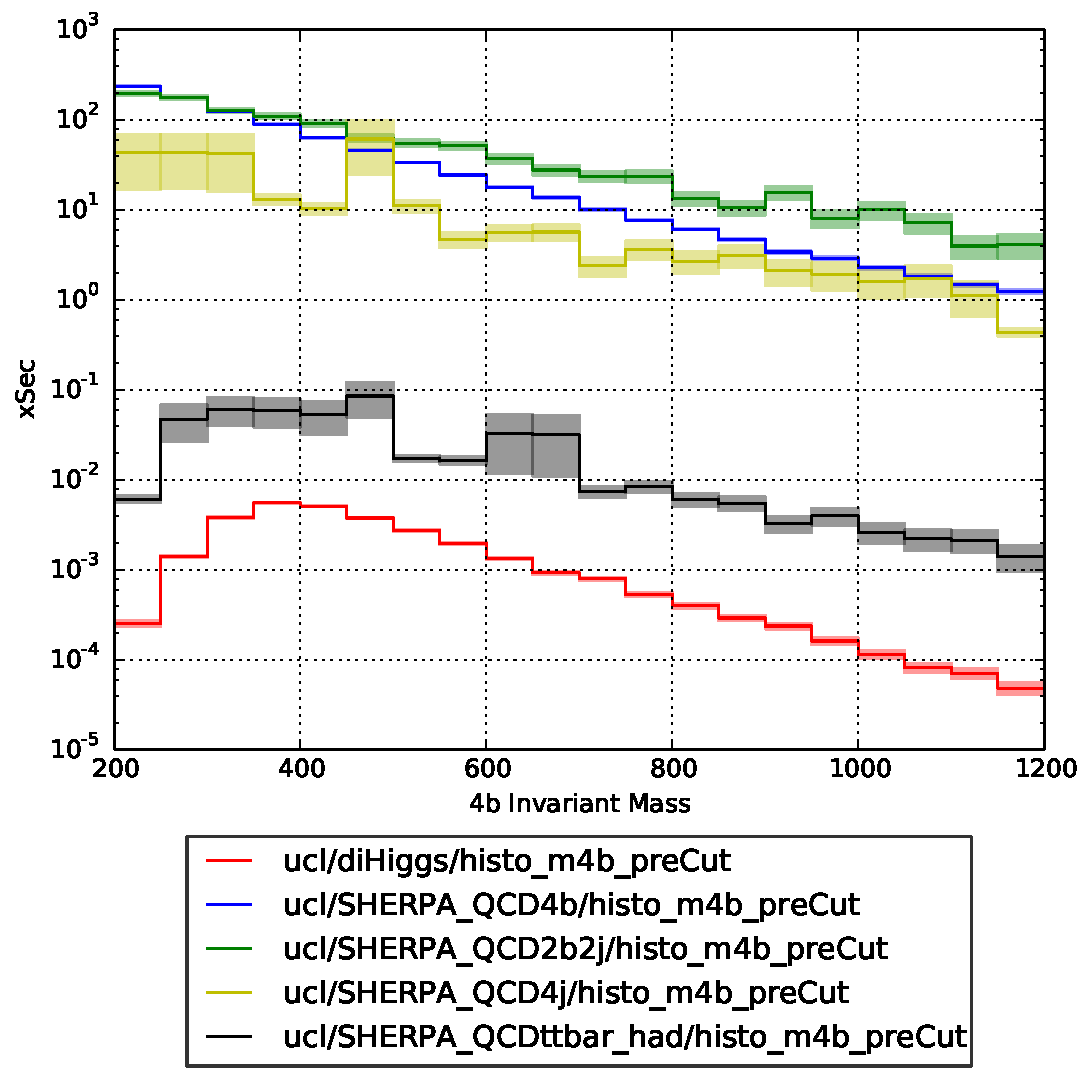
\includegraphics[width=\textwidth]{plots/m4b_ucl_preCut.pdf}
\caption{Contributions from the various samples to the observed four $b$ invariant mass system after applying the $b$-tagging procedure outlined in Section~\ref{sec:btagtest}.}
\end{center}
\end{figure}


\subsubsection{$bb$-jet rejection for the four hardest jets}

\begin{figure}[h!]
\begin{center}
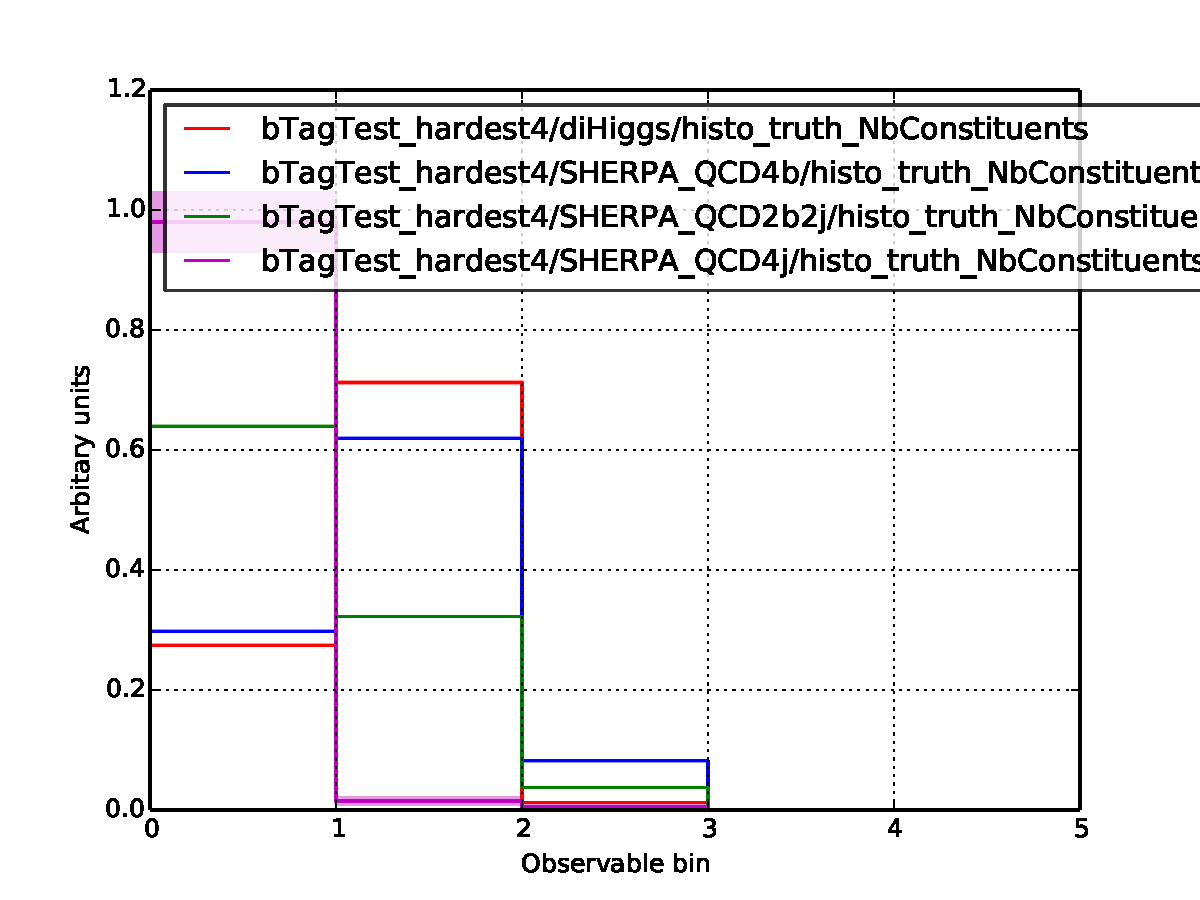
\includegraphics[width=\textwidth]{plots/histo_NbConstits_4hardest.pdf}
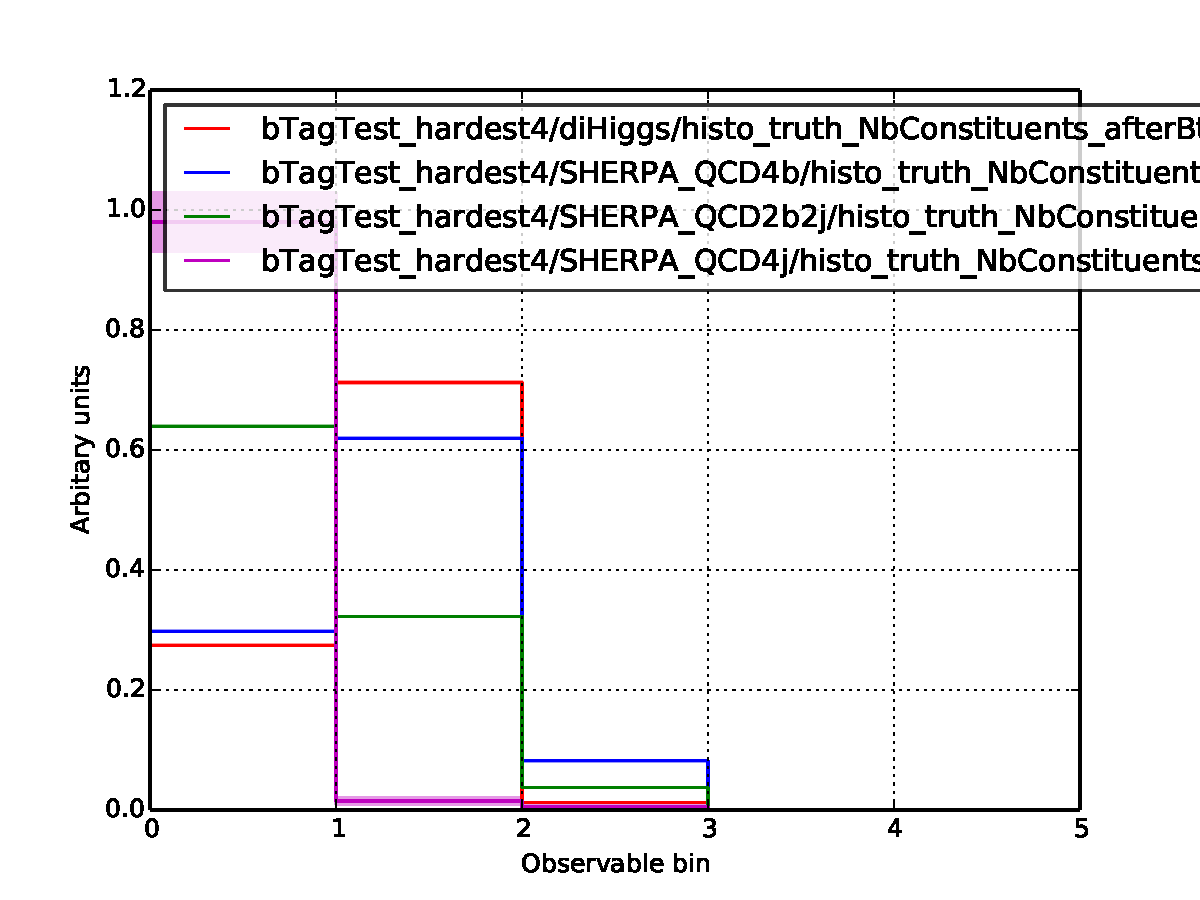
\includegraphics[width=\textwidth]{plots/histo_NbConstits_4hardest_afterBtag.pdf}
\caption{.}
\end{center}
\end{figure}

\begin{table}[h]
\begin{center}
\begin{tabular}{|c|c|c|c|c|}
\hline
Process & $\sigma_{\mathrm{tot}}$ (4 Jets $p_T>40$ GeV) & After b-tag & After $bb$ rejection & \% selected  \\
\hline \hline
$H\bar{H}$ & 17.2911 & 1.4655 & 1.38429 & \% \\
\hline
$b\bar{b}b\bar{b}$ & 1.12149e+06 & 101152 & 95723.1 & \% \\
$b\bar{b}jj$ & 2.65895e+08 & 98116.7 & 88956.2 & \% \\
$jjjj$ & 1.22738e+10 & 626267 & 604.205 & \% \\
\hline
\textbf{S/B} & & & & \multicolumn{1}{c}{}\\
\cline{1-3}
\textbf{S/$\sqrt{\mathrm{\textbf{B}}}$}& & & & \multicolumn{1}{c}{}\\
\cline{1-3}
\end{tabular}
\end{center}
\caption{Summary of the $b$-tagging and $bb$-rejection cuts on the four leading jets.}\label{tab:TestbbTag}
\end{table}%


\subsubsection{$bb$-jet rejection for the UCL-style selection}

\begin{figure}[h!]
\begin{center}
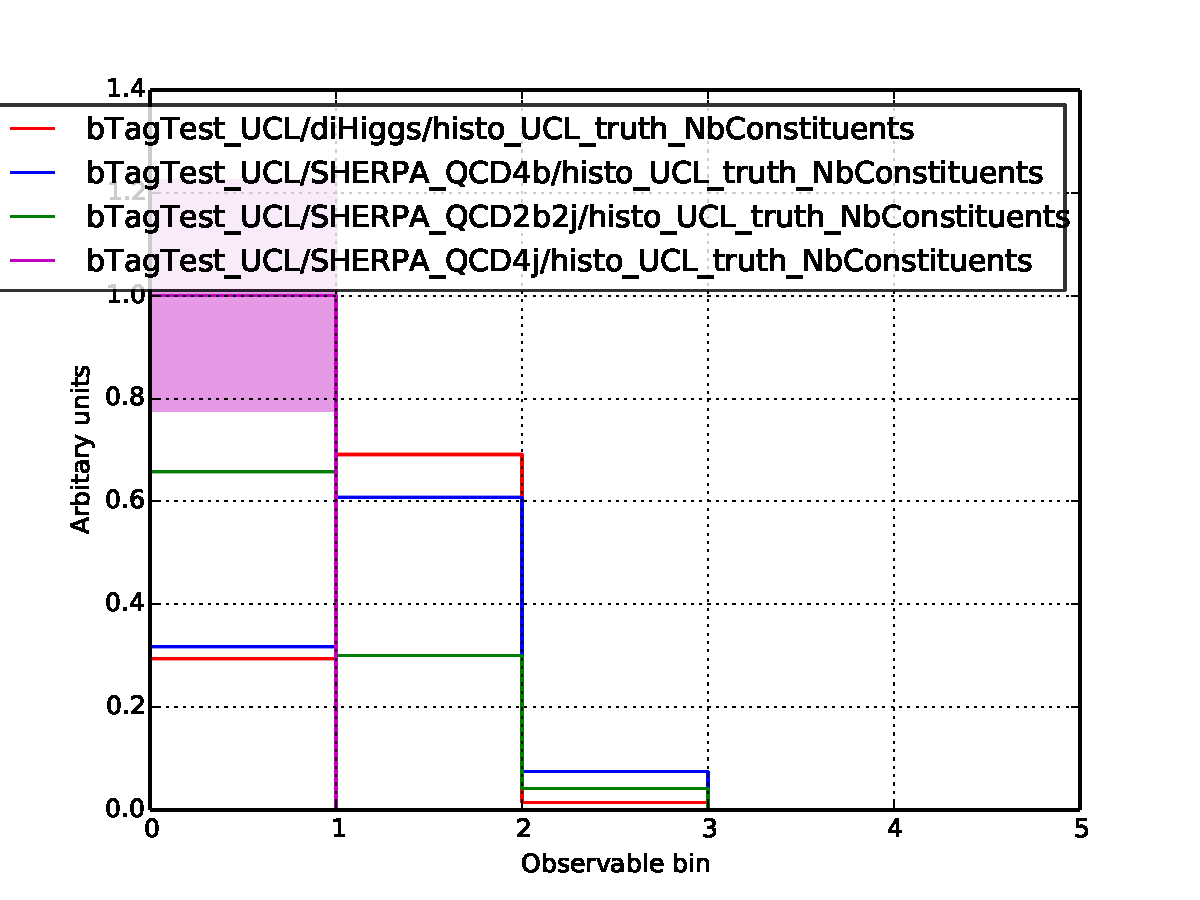
\includegraphics[width=\textwidth]{plots/histo_NbConstits_UCL.pdf}
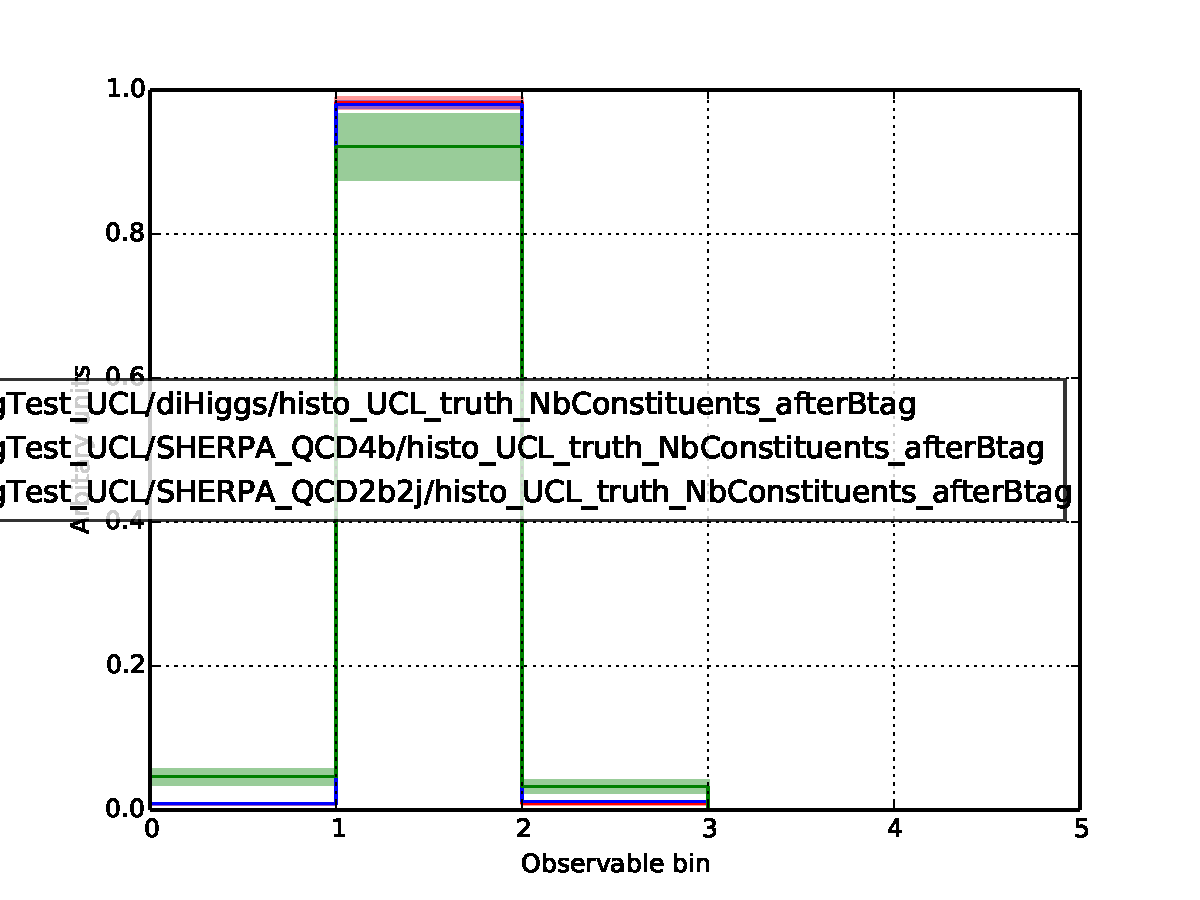
\includegraphics[width=\textwidth]{plots/histo_NbConstits_UCL_afterBtag.pdf}
\caption{.}
\end{center}
\end{figure}

\begin{table}[h]
\begin{center}
\begin{tabular}{|c|c|c|c|c|}
\hline
Process & $\sigma_{\mathrm{tot}}$ (4 Jets $p_T>40$ GeV) & After b-tag & After $bb$ rejection & \% selected  \\
\hline \hline
$H\bar{H}$ &10.7756 & 0.796946 & 0.744208 & 7.467\% \\
\hline
$b\bar{b}b\bar{b}$ & 101152 & 4789.57 & 4438.72 & \% \\
$b\bar{b}jj$ & 1.72539e+07 & 9962.27 & 8564.06 & \% \\
$jjjj$ & 6.10999e+08 & 1.07288e-06 & 1.07288e-06 & \% \\
\hline
\textbf{S/B} & & & & \multicolumn{1}{c}{}\\
\cline{1-3}
\textbf{S/$\sqrt{\mathrm{\textbf{B}}}$} & & & & \multicolumn{1}{c}{}\\
\cline{1-3}
\end{tabular}
\end{center}
\caption{Summary of the $b$-tagging and $bb$-rejection cuts on the four leading jets.}\label{tab:TestbbTagUCL}
\end{table}%



\subsection{Boosted Topology}\label{sec:Boosted_FR}

In the boosted topology, the decay products of each Higgs boson are merged into a single large-$R$ jet with a two-prong substructure. 
These Higgs jets are reconstructed as anti-$k_T$ $R=1.0$ jets for which two substructure variables, the first $k_T$ splitting scale $d_{12}$
and the 2-subjettiness ratio $\tau_{21}$, are calculated.
\textit{Pre-cut} histograms are written out after requiring the presence of at least two large-$R$ in the event but without applying any further
kinematic cuts. \textit{Post-cut} histograms are filled after the following additional cuts: 
Both jets are required to have $p_T >$100~GeV and $|\eta|>2.5$. Moreover, each jet is required to have at least two b-tagged anti-$k_T$ $R=0.3$ 
jets matched to it via \textit{ghost association}: 
To this end, the constituents of a given large-$R$ jet is reclustered using the jet algorithm 
and radius parameter of the original jet and so-called \textit{ghost jets}, each corresponding to a small-$R$ jet in the event, 
are added to the input for the cluster sequence. The 4-vector of a ghost jet is obtained from a given small-$R$ jet 
by setting its transverse momentum and mass to negligibly small values but retaining its direction in $\eta$ and $\phi$. A small-$R$ jet is 
considered matched to the large-$R$ jet if its ghost is found among the constituents of the reclustered jet. Ghost association allows to unambiguously
match small-$R$ to large-$R$ jets, even in dense environments where a simple matching based on the distance $\Delta R$ between jets 
may lead to multiple matchings.

\begin{figure}[h]
\begin{center}
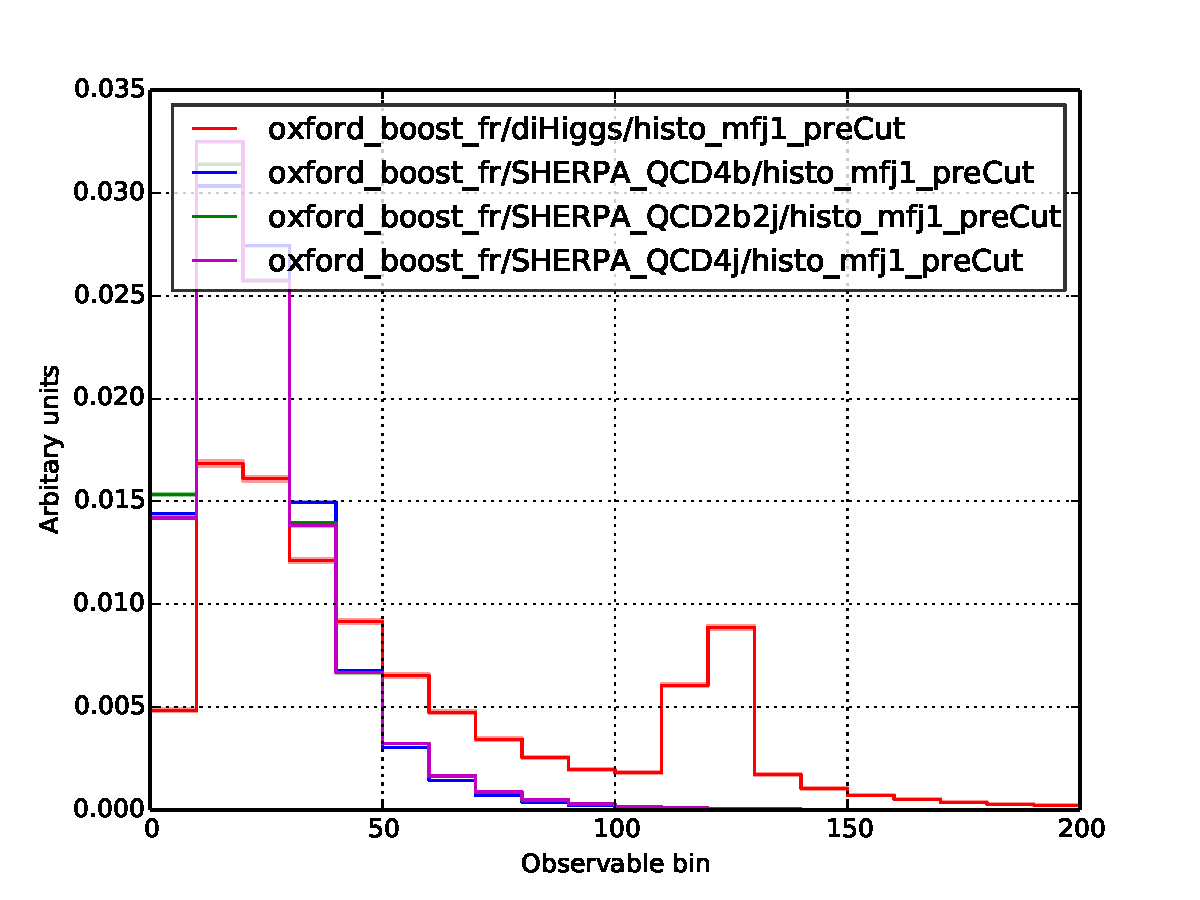
\includegraphics[width=0.49\textwidth]{plots/histo_mfj1_preCut.pdf}
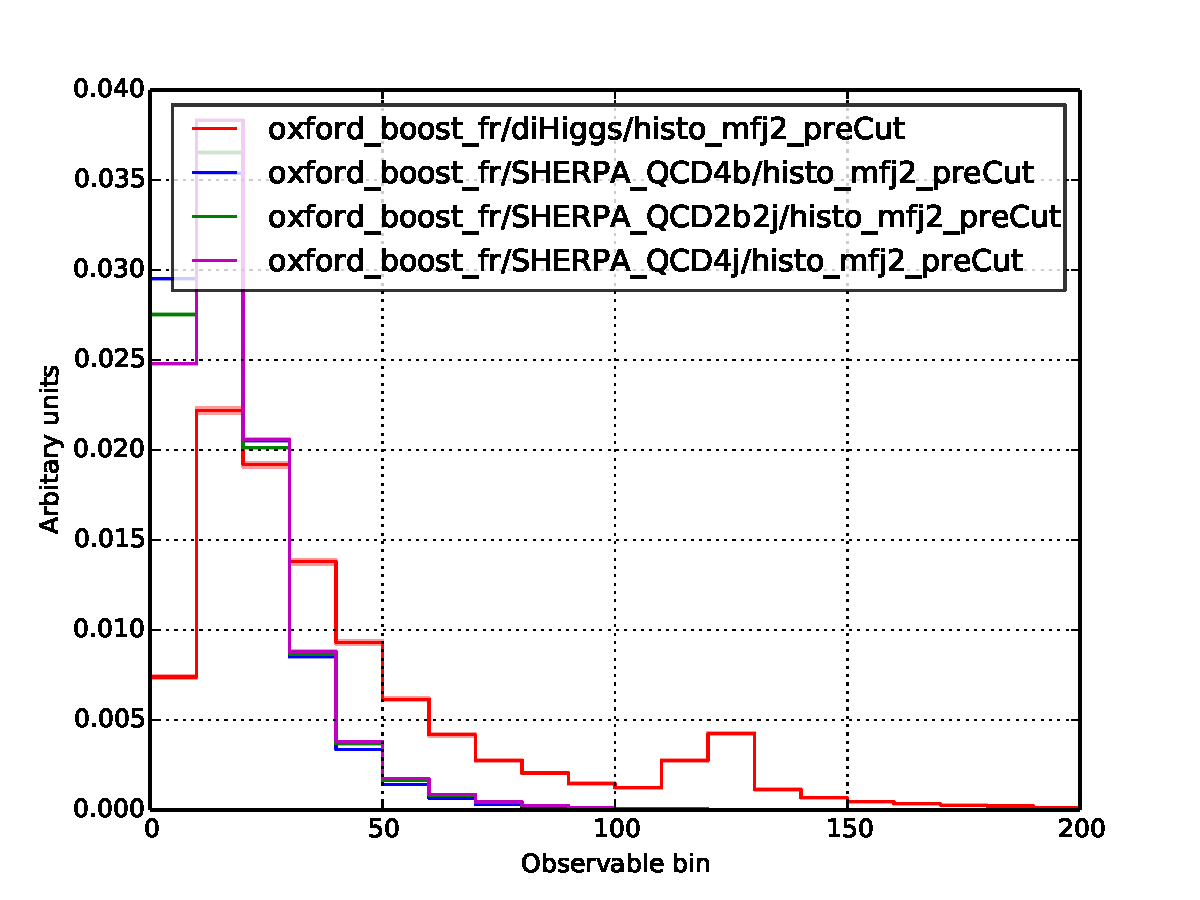
\includegraphics[width=0.49\textwidth]{plots/histo_mfj2_preCut.pdf}
\caption{Mass distributions for the leading and subleading anti-$k_T$ $R=1.0$ jets before the applying the boosted selection.}
\label{fig:mfj_boosted_pre}
\end{center}
\end{figure}

\begin{figure}[h]
\begin{center}
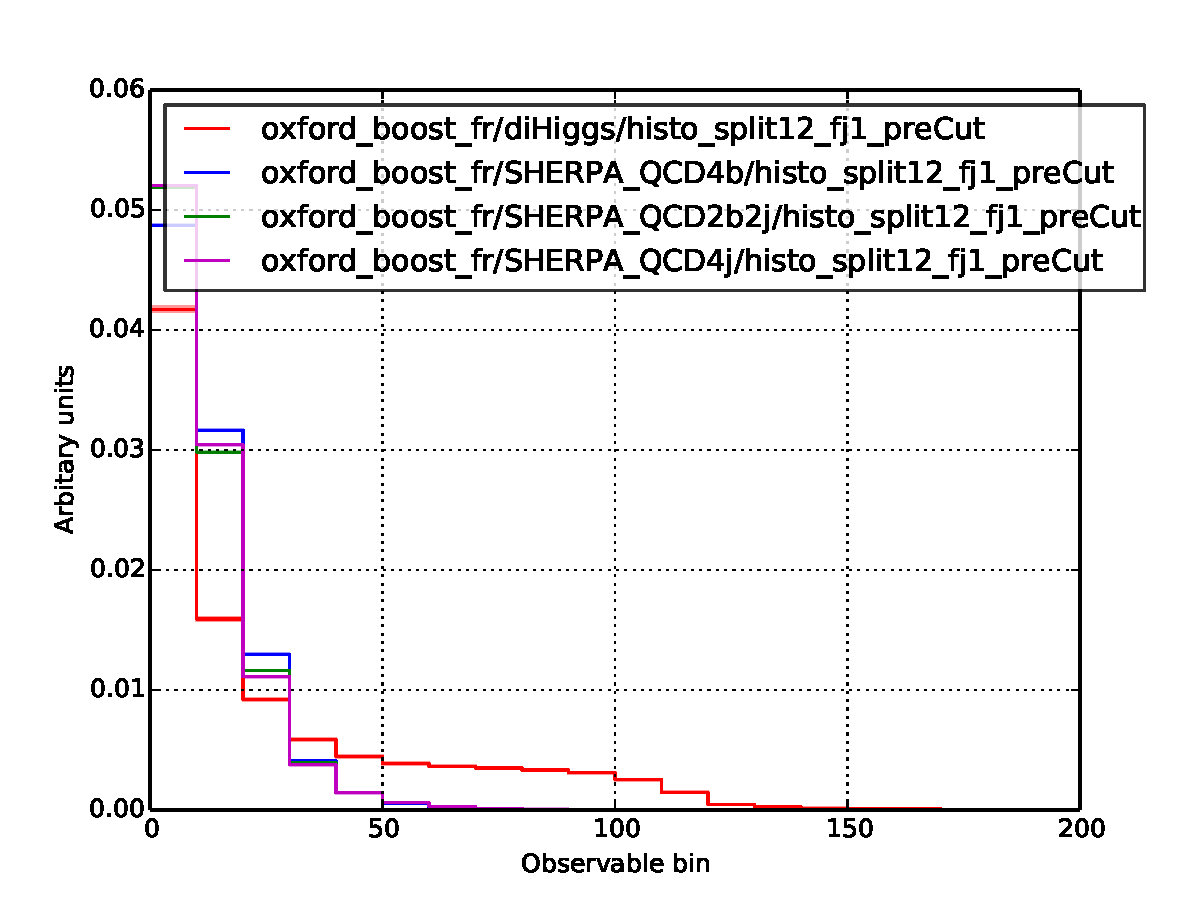
\includegraphics[width=0.49\textwidth]{plots/histo_split12_fj1_preCut.pdf}
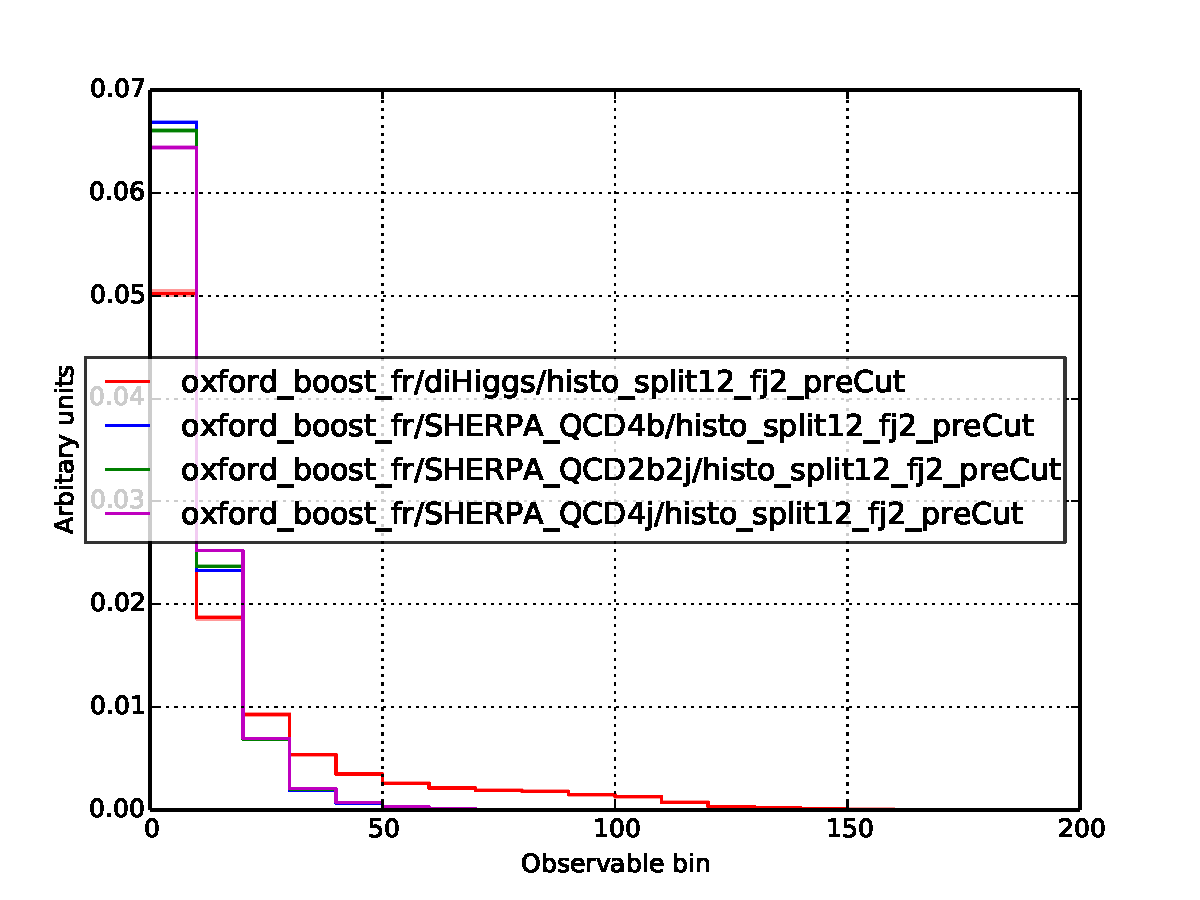
\includegraphics[width=0.49\textwidth]{plots/histo_split12_fj2_preCut.pdf}
\caption{$d_{12}$ distributions for the leading and subleading anti-$k_T$ $R=1.0$ jets before the applying the boosted selection.}
\label{fig:split12_fj_boosted_pre}
\end{center}
\end{figure}

\begin{figure}[h]
\begin{center}
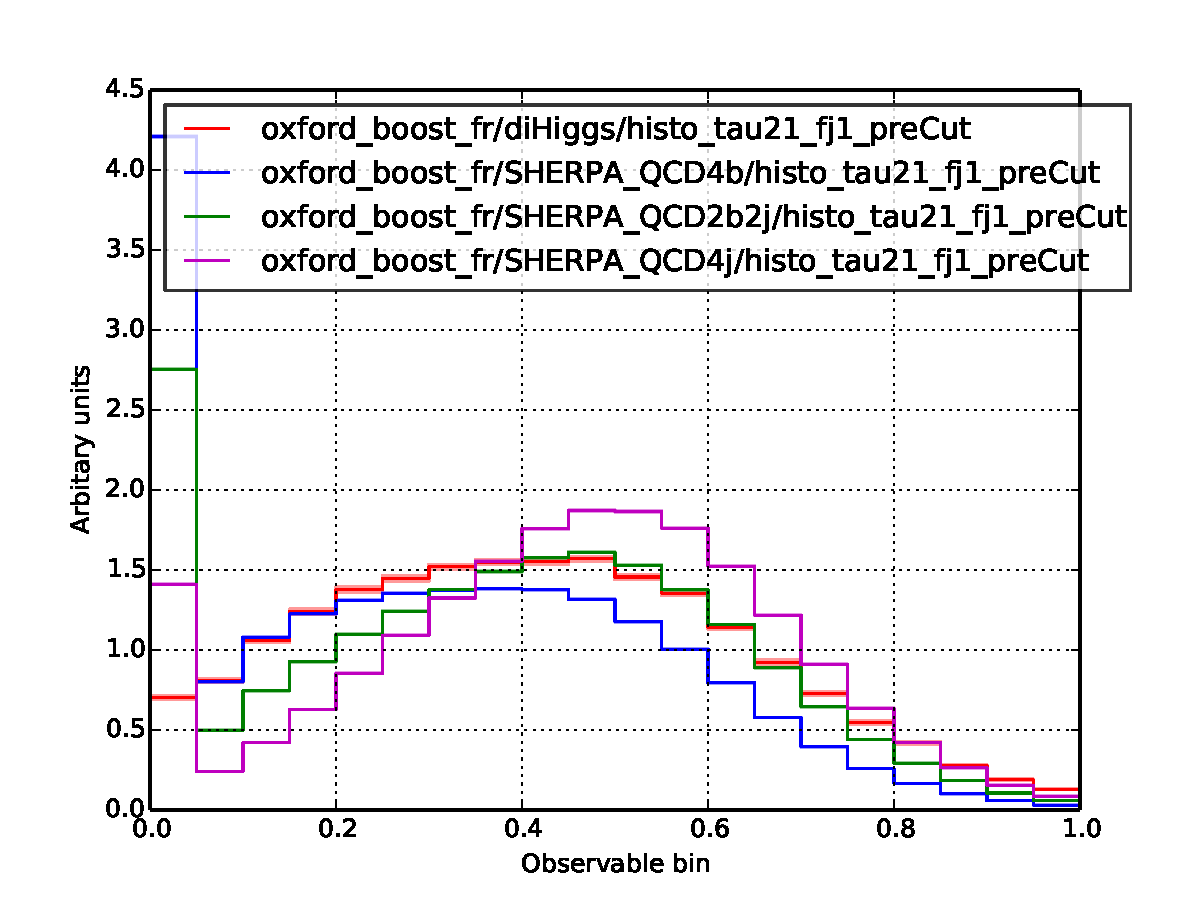
\includegraphics[width=0.49\textwidth]{plots/histo_tau21_fj1_preCut.pdf}
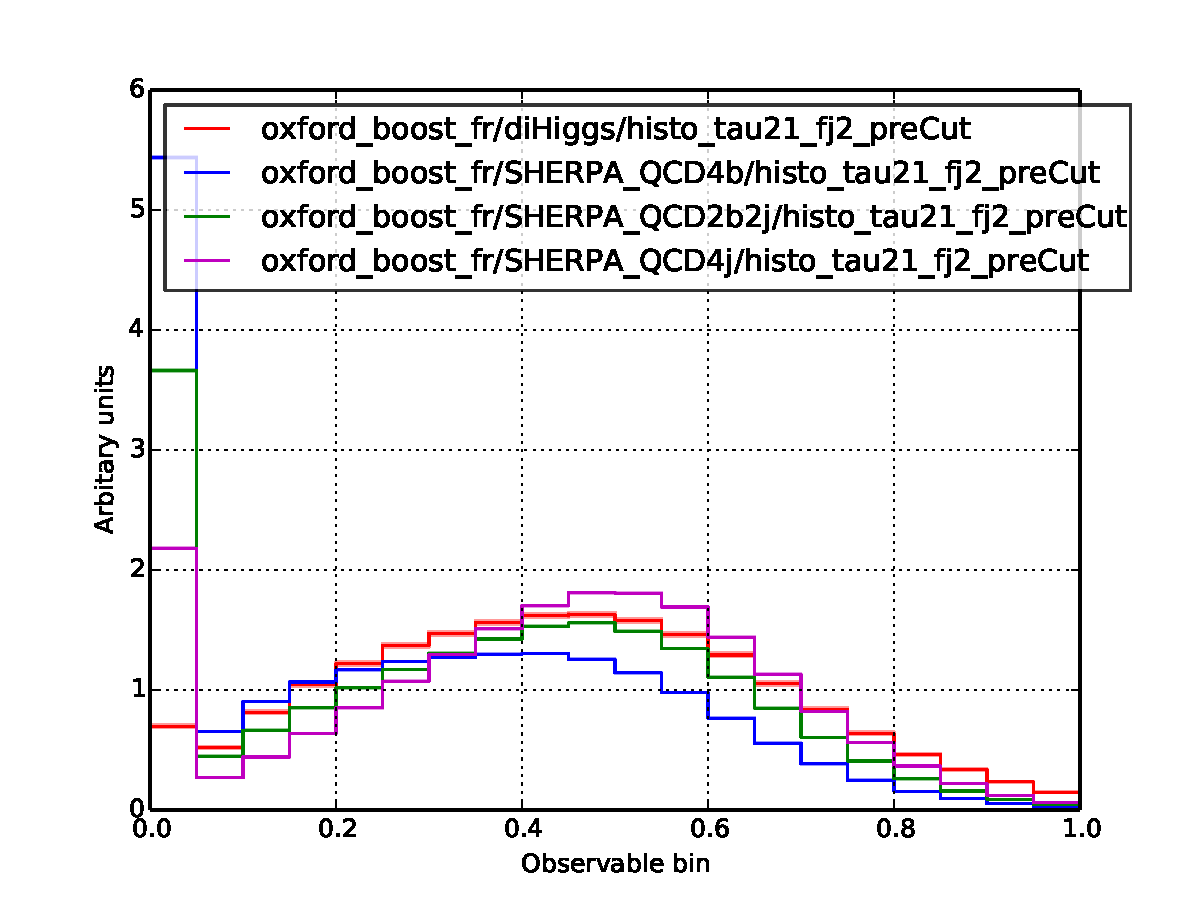
\includegraphics[width=0.49\textwidth]{plots/histo_tau21_fj2_preCut.pdf}
\caption{$\tau_{21}$ distributions for the leading and subleading anti-$k_T$ $R=1.0$ jets before the applying the boosted selection.}
\label{fig:tau21_fj_boosted_pre}
\end{center}
\end{figure}

\begin{figure}[h]
\begin{center}
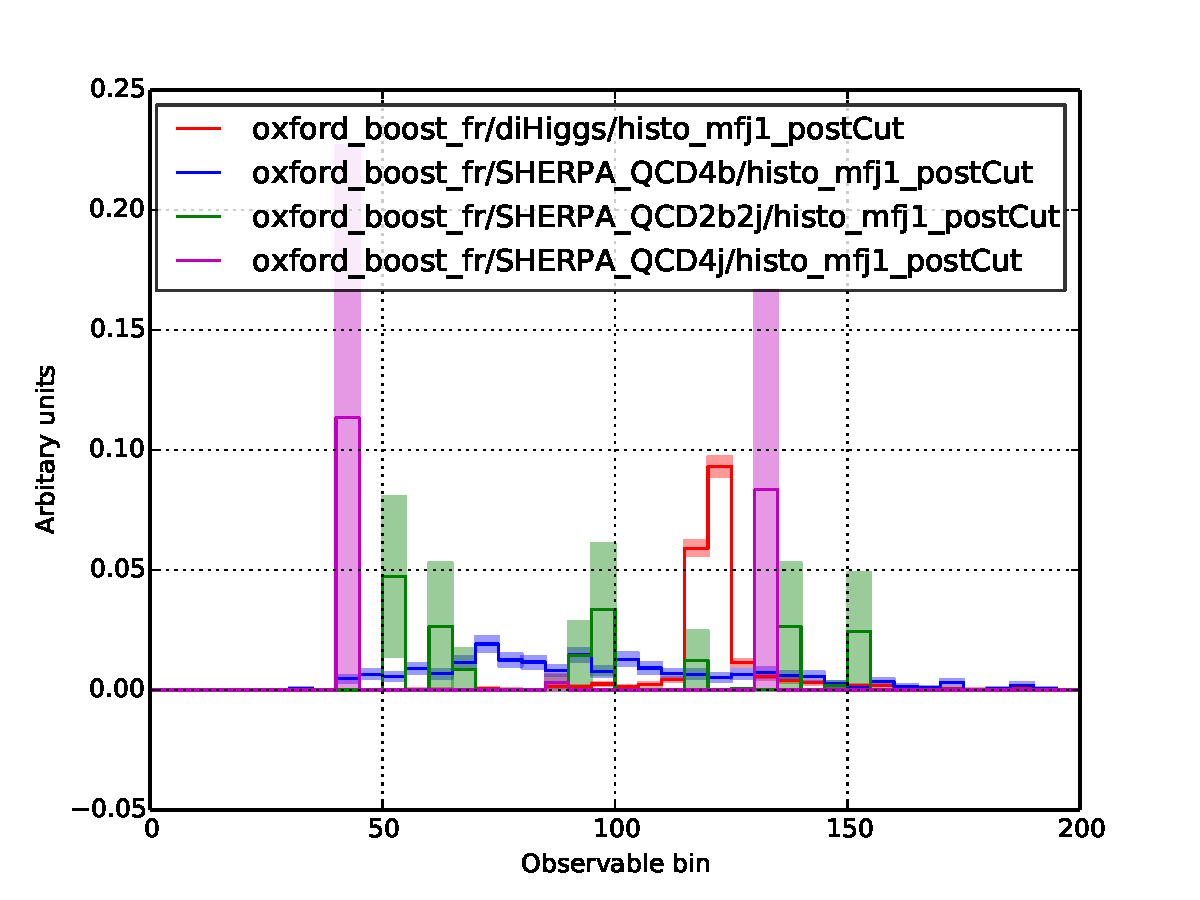
\includegraphics[width=0.49\textwidth]{plots/histo_mfj1.pdf}
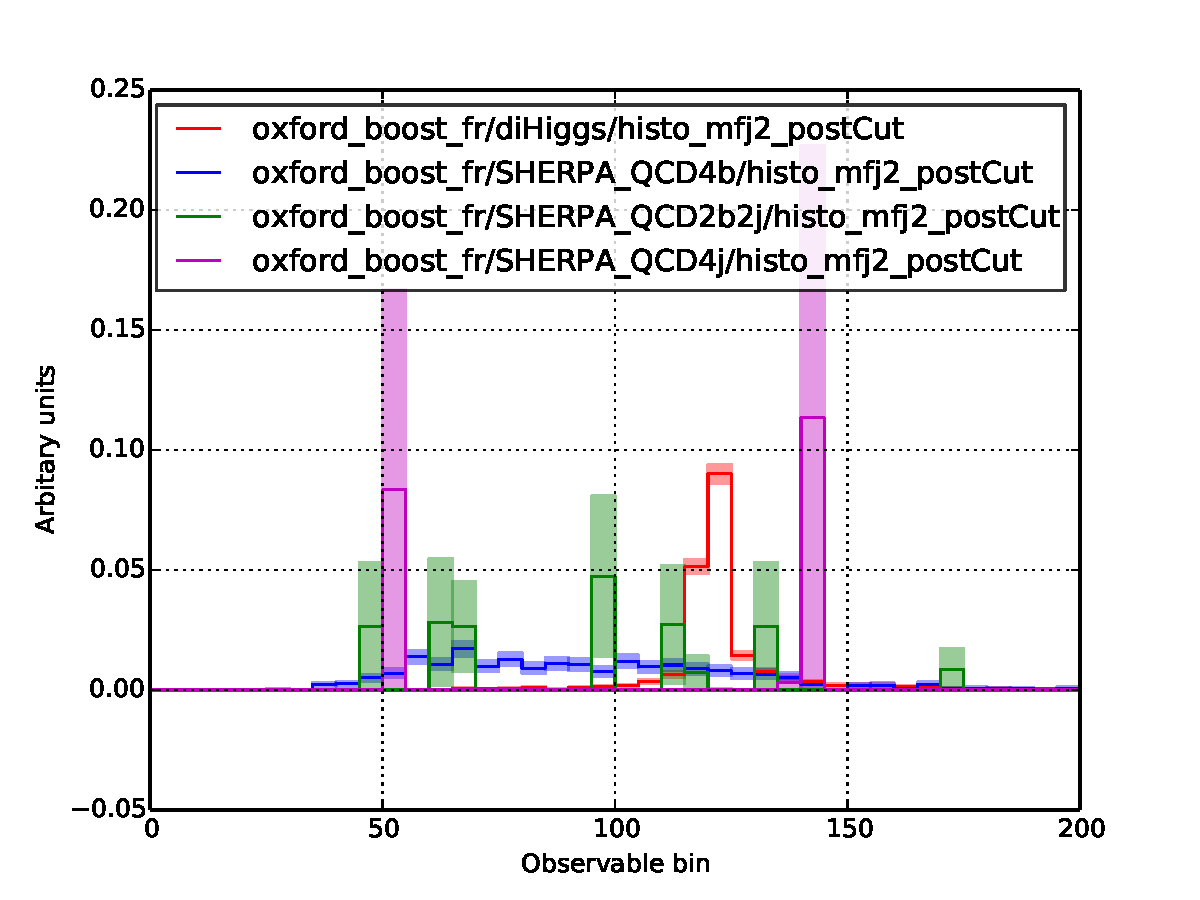
\includegraphics[width=0.49\textwidth]{plots/histo_mfj2.pdf}
\caption{Mass distributions for the leading and subleading anti-$k_T$ $R=1.0$ jets after the applying the boosted selection.}
\label{fig:mfj_boosted_post}
\end{center}
\end{figure}

\begin{figure}[h]
\begin{center}
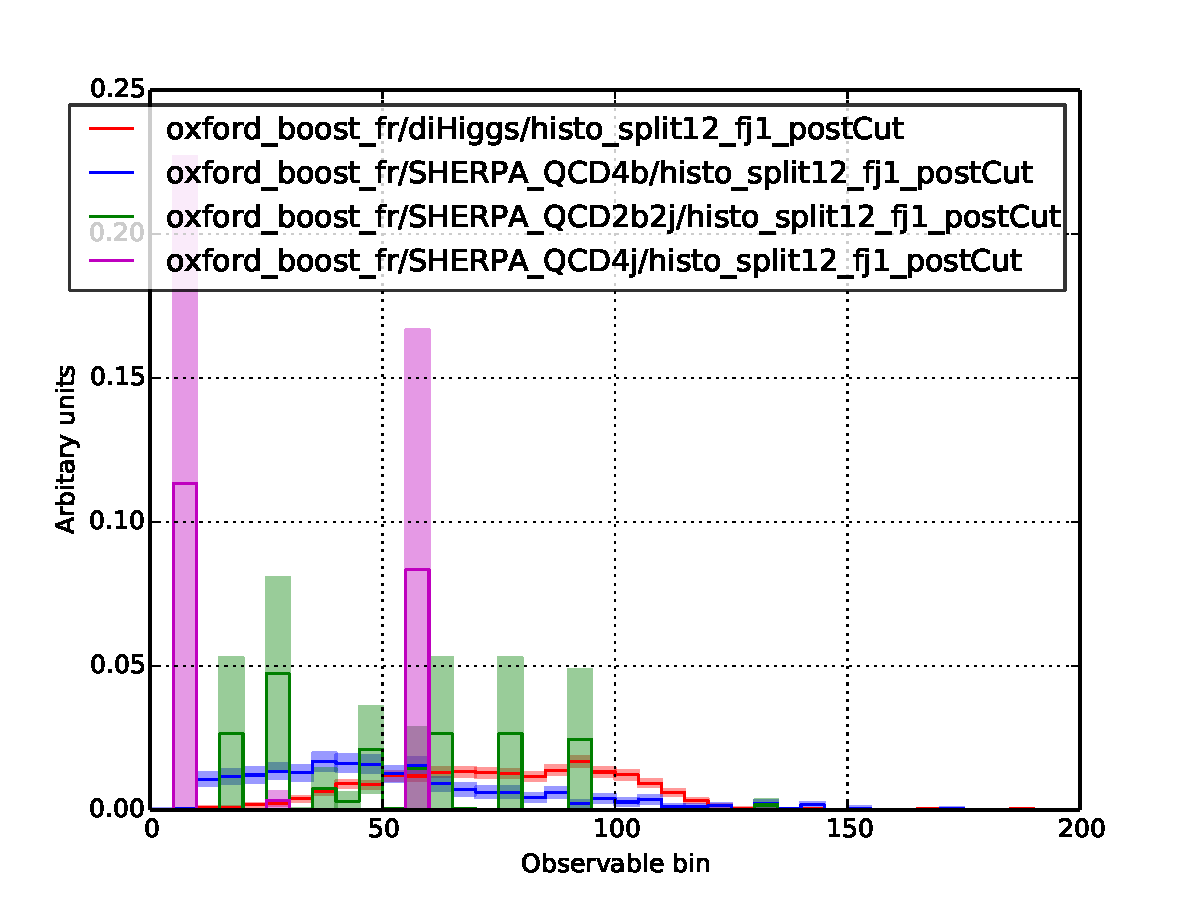
\includegraphics[width=0.49\textwidth]{plots/histo_split12_fj1.pdf}
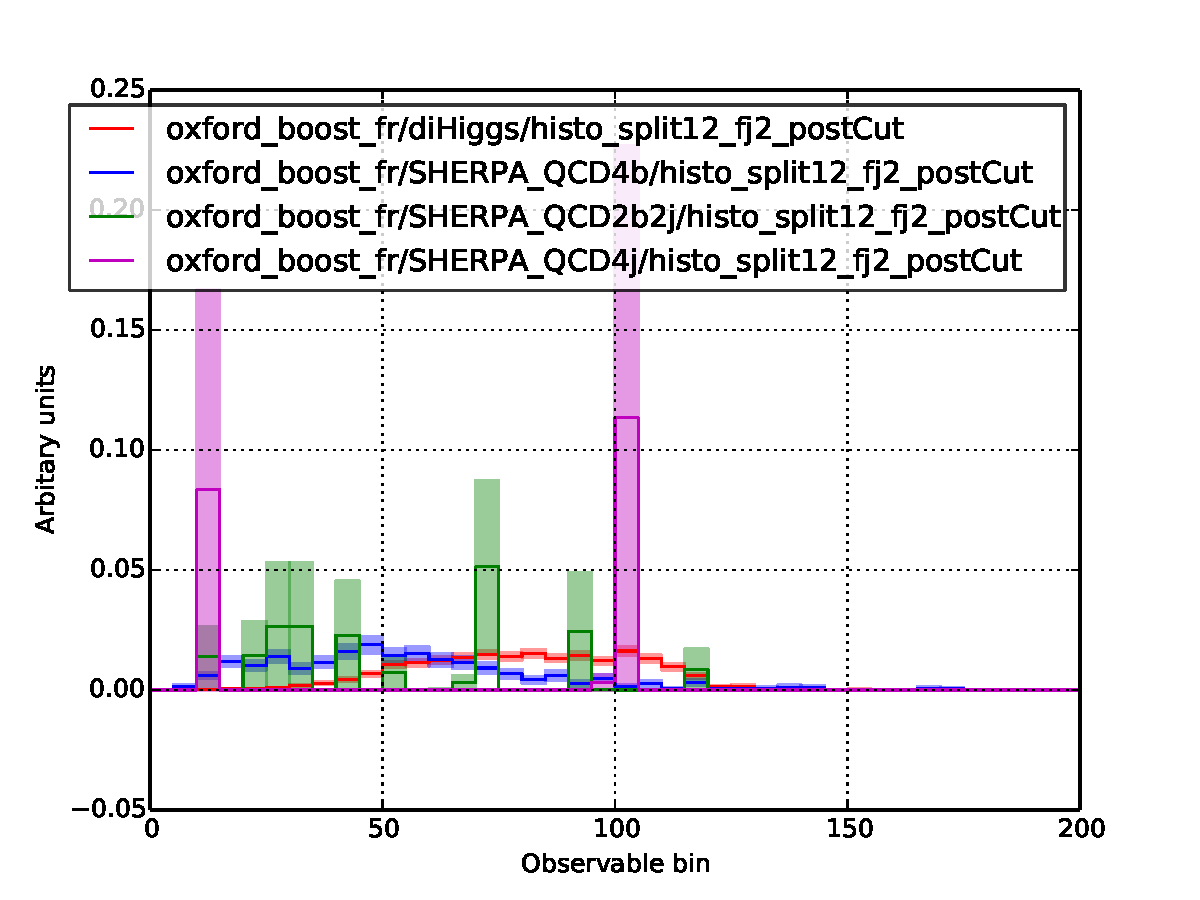
\includegraphics[width=0.49\textwidth]{plots/histo_split12_fj2.pdf}
\caption{$d_{12}$ distributions for the leading and subleading anti-$k_T$ $R=1.0$ jets after the applying the boosted selection.}
\label{fig:split12_fj_boosted_post}
\end{center}
\end{figure}

\begin{figure}[h]
\begin{center}
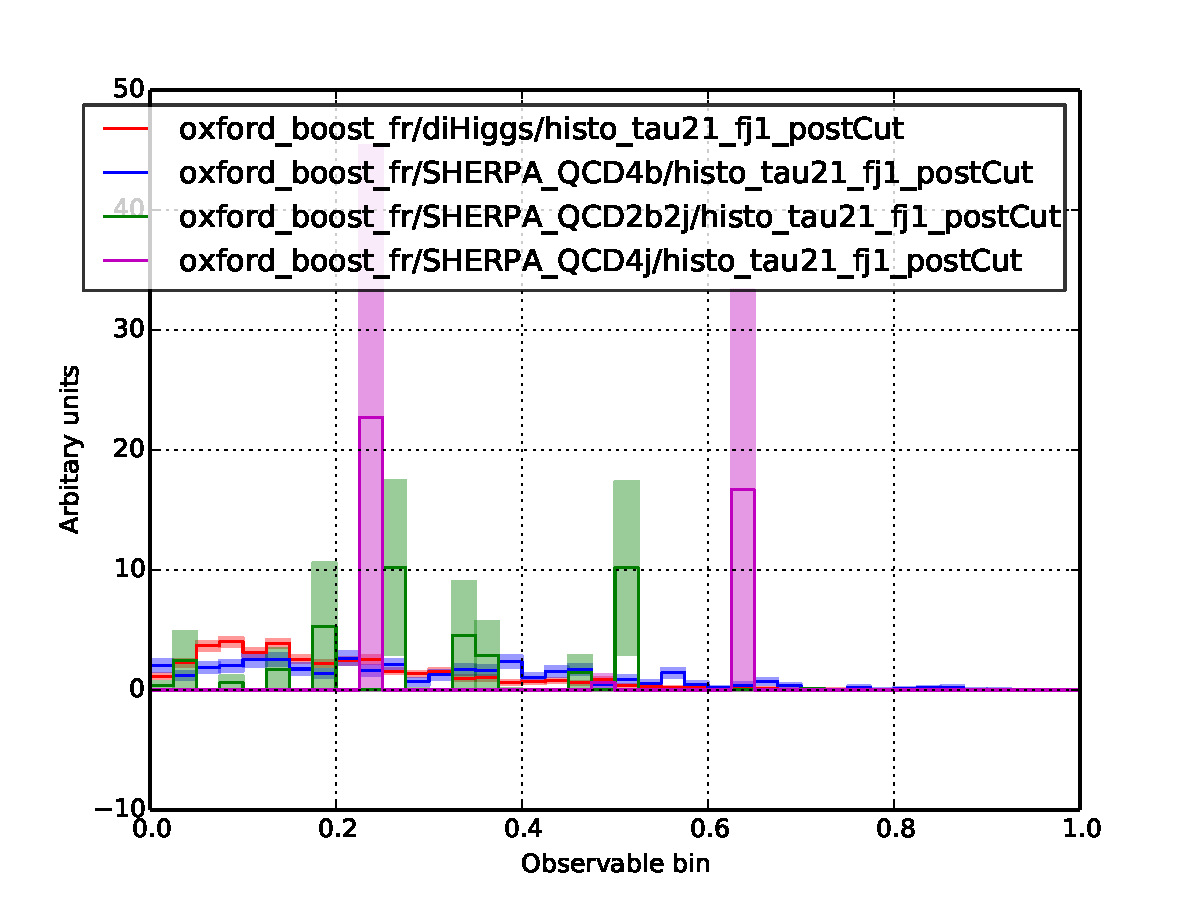
\includegraphics[width=0.49\textwidth]{plots/histo_tau21_fj1.pdf}
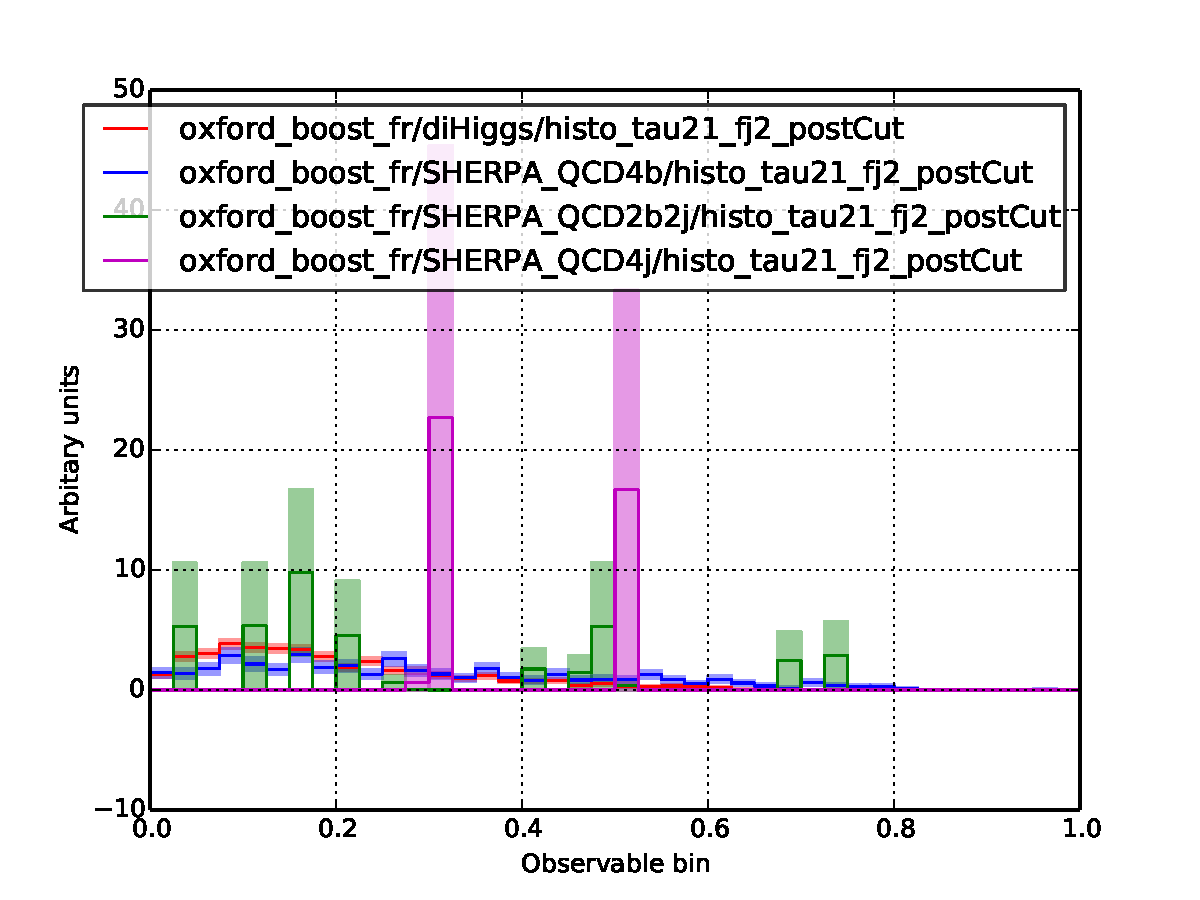
\includegraphics[width=0.49\textwidth]{plots/histo_tau21_fj2.pdf}
\caption{$\tau_{21}$ distributions for the leading and subleading anti-$k_T$ $R=1.0$ jets after the applying the boosted selection.}
\label{fig:tau21_fj_boosted_post}
\end{center}
\end{figure}

\subsection{Boosted Topology with Variable-$R$ Jets}

The same selection as in Subsection~\ref{sec:Boosted_FR} is applied but this time using Variable-$R$ jets with the following parameters:
$\rho=500$~GeV, $R_{max}=$1.0, $R_{min}=$0.2.

\section{Multivariate Tools}

\clearpage
\section{Results}
\subsection{Example resolved analysis}
In this section we present the results of a resolved style analysis upon the full set of available samples for the purposes of illustration. The cuts used in this example analysis are as so. \emph{b-tag} cuts those events which fail to tag four anti-$k_T$ $R=0.5$ $b$-jets with $b$ quark $p_T > 15$ GeV. Flat $b$-jet efficiencies and mistag rates of 80\% and 1\% respectively. A $c$ mistag rate of $17\%$ is also applied.  \emph{jet $p_T$,$\eta$} requires that the four jets each have $p_T>40$ GeV and $|\eta|< 2.5$. \emph{di-jet $p_T$} requires that each dijet pair representing a higgs candidate has $p_T>150 $ GeV. \emph{di-jet $\Delta\eta$} requires that the two dijets are separated by no more than 1.5 units in $\eta$. Finally \emph{$m_H$ window} requires that the invariant mass of each dijet is within 15 GeV of $m_H$. The remaining cross-section after each of these cuts, along with $S/B$ and $S/\sqrt{B}$ are given in Table ~\ref{tab:resCutflow}.

\begin{table}[htdp]
\begin{center}
\begin{tabular}{|c||c||c|c|c|c||c|c|}
\hline
Cut 					& $HH$ [fb] & $4b$ [fb] & $2b2j$ [fb] & $4j$ [fb] & $t\bar{t}$ [fb] & $S/B$ & $S/\sqrt{B}$ \\
\hline
\hline
b-tag    	& 1.516 &      102271         & 135255        & 42934  	&	202.9	&5.40E-6	& 0.157\\
jet $p_T,\eta$         & 0.723 &        3847      & 10676       & 5045 	&	122.7	&3.67E-5	& 0.282\\
di-jet $p_T$           	& 0.371&      553.7        & 1838	  & 926.0	&	22.45	&1.11E-4	& 0.352\\
di-jet $\Delta\eta$   & 0.336&       324.8       & 991.4 	  & 312.6		&	16.39	&2.04E-4	& 0.454\\
\hline
$m_H$ window   &0.190 &          7.632      & 13.60	  & 0.502	&	2.675	&7.78E-3	& 2.106\\
\hline
\end{tabular}
\end{center}
\caption{Table demonstrating the cutflow of an example resolved analysis applied to the full sample set.  $S/\sqrt{B}$ is given for HL-LHC luminosities.}
\label{tab:resCutflow}
\end{table}%


\subsection{Example boosted analysis}
Here we shall discuss an example boosted analysis. In this case \emph{Fatjet cuts} refers to the requirement of two $R=1$ anti-$k_T$ jets with $p_T>250$ GeV and $|\eta| < 2.5$. \emph{2 Subjets} requires two anti-$k_T$ $R=0.3$ subjects in each fat jet. \emph{b-Tagging} cuts those events in which the two hardest subjets are not successfully $b$-tagged. Here efficiency and mistag factors are applied for $b$ and $c$ jets as a function of subjet $p_T$. \emph{Mass-drop } requires that the two fat jets pass a BDRS mass-drop tagger with parameters $\mu = 0.67$ and $y_{\mathrm{cut}} = 0.09$. Finally \emph{$m_H$ window} only passes events where the two fat jet masses are within $15$ GeV of $m_H$. In Table~\ref{tab:boostedCutflow} we see the results of these cuts.
\begin{table}[htdp]
\begin{center}
\begin{tabular}{|c||c||c|c|c|c||c|c|}
\hline
Cut 					& $HH$ [fb] & $4b$ [fb] & $2b2j$ [fb] & $4j$ [fb] & $t\bar{t}$ [fb] & $S/B$ & $S/\sqrt{B}$ \\
\hline
\hline
Fatjet cuts 			&2.802           	&3045 	& 1.13E6 &	4.57E7    &       9808  & 5.98E-8 &0.022 \\
2 Subjets  	&	2.740 	&2694	& 1.01E6	&	4.21E7 	&	9787  &6.35E-8 & 0.023\\
b-Tagging    			& 0.070		&39.76	& 296.9		&	352.9            &      7.586 & 1.00E-5& 0.145\\
Mass-drop  		& 0.068 		&36.84	& 256.0    	&	305.1            &	7.514 & 1.12E-4& 0.151 \\
\hline
$m_H$ window       		&   0.045		& 2.134	& 10.83	& 	0.630            & 	0.438 & 3.20E-3& 0.658\\
\hline
\end{tabular}
\end{center}
\caption{Table demonstrating the cutflow of an example boosted analysis applied to the full sample set. $S/\sqrt{B}$ is given for HL-LHC luminosities.}
\label{tab:boostedCutflow}
\end{table}%


\subsection{MVA}
We now apply a basic MVA to the final output of the resolved and boosted analyses. The MVA used is a feedforward artificial neural network with $N_{\mathrm{par}}\times5\times3\times1$ architecture, where $N_{\mathrm{par}}$ is the number of input parameters for the network. The MVA was trained for 50,000 GA generations with a cross-entropy error function. In Figure~\ref{fig:nnresponse} the neural network classification of events is demonstrated for both the resolved and boosted cases. In Figure~\ref{fig:exampleroc} the ROC curves for the two analyses are shown, demonstrating that the neural network is able to
perform well in both cases. Figure~\ref{fig:nnweights} shows the distribution of NN weights in both cases.


\begin{figure}[h]
\begin{center}
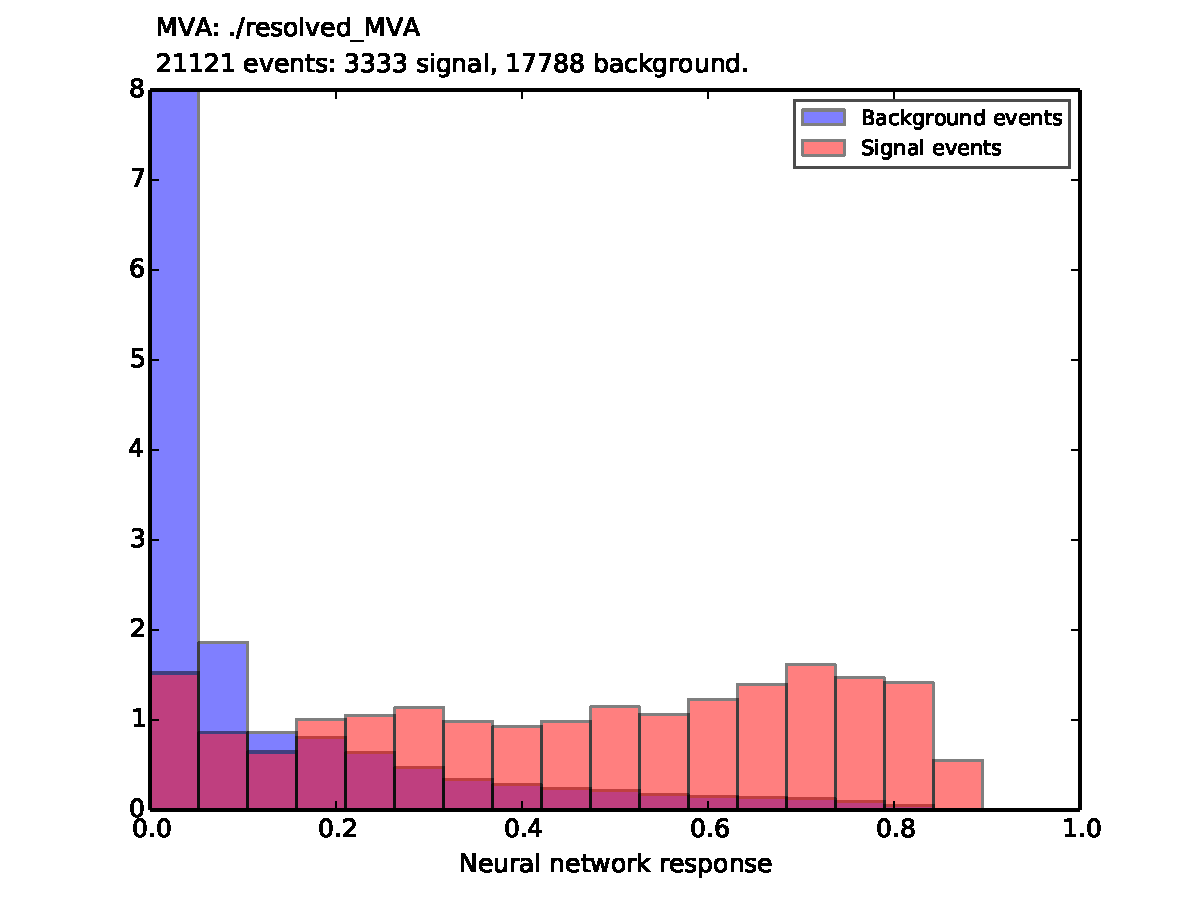
\includegraphics[width=0.49\textwidth]{plots/resolved_MVA_hist.pdf}
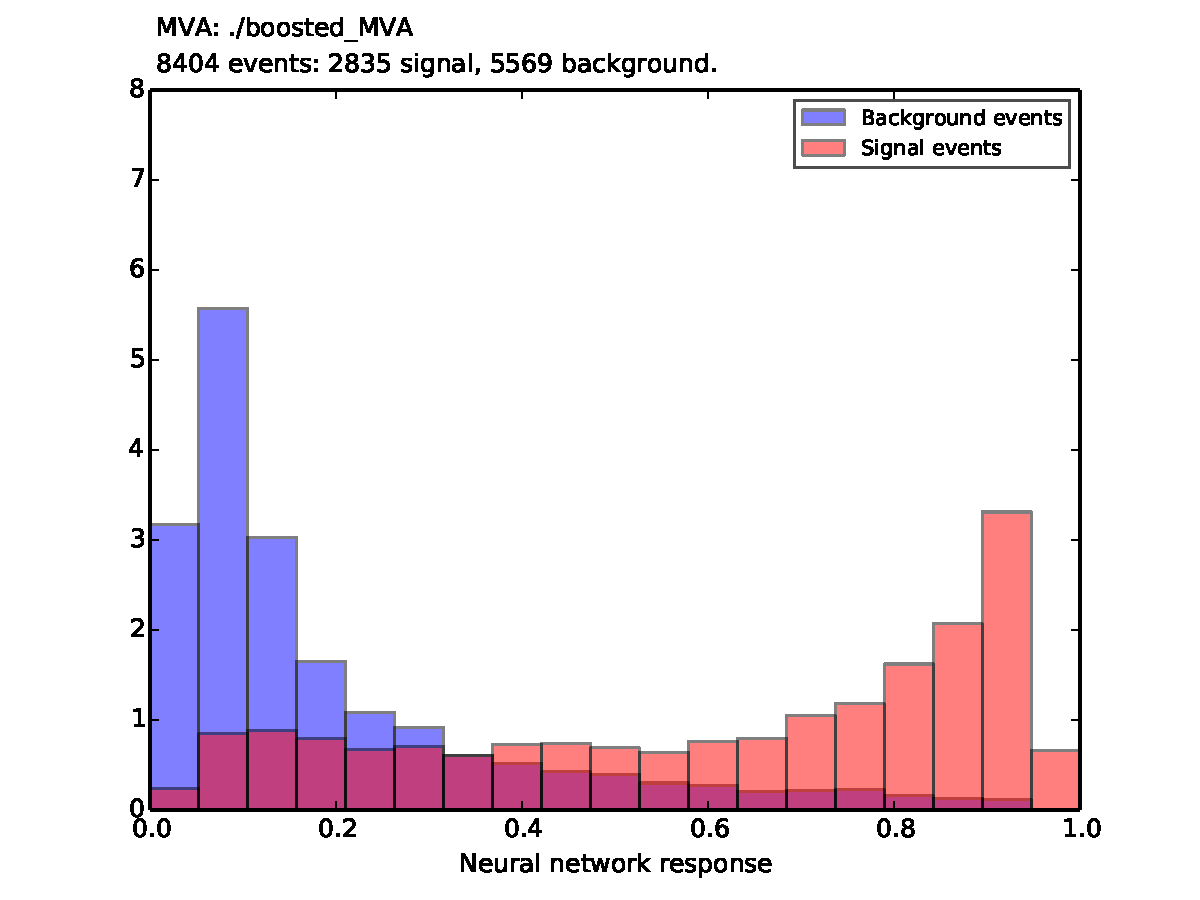
\includegraphics[width=0.49\textwidth]{plots/boosted_MVA_hist.pdf}
\caption{Neural network response demonstrated for the case of the resolved (left) and boosted (right) analyses. The frequency of background and signal events is plotted as a function of neural network output.}
\label{fig:nnresponse}
\end{center}
\end{figure}

\begin{figure}[h]
\begin{center}
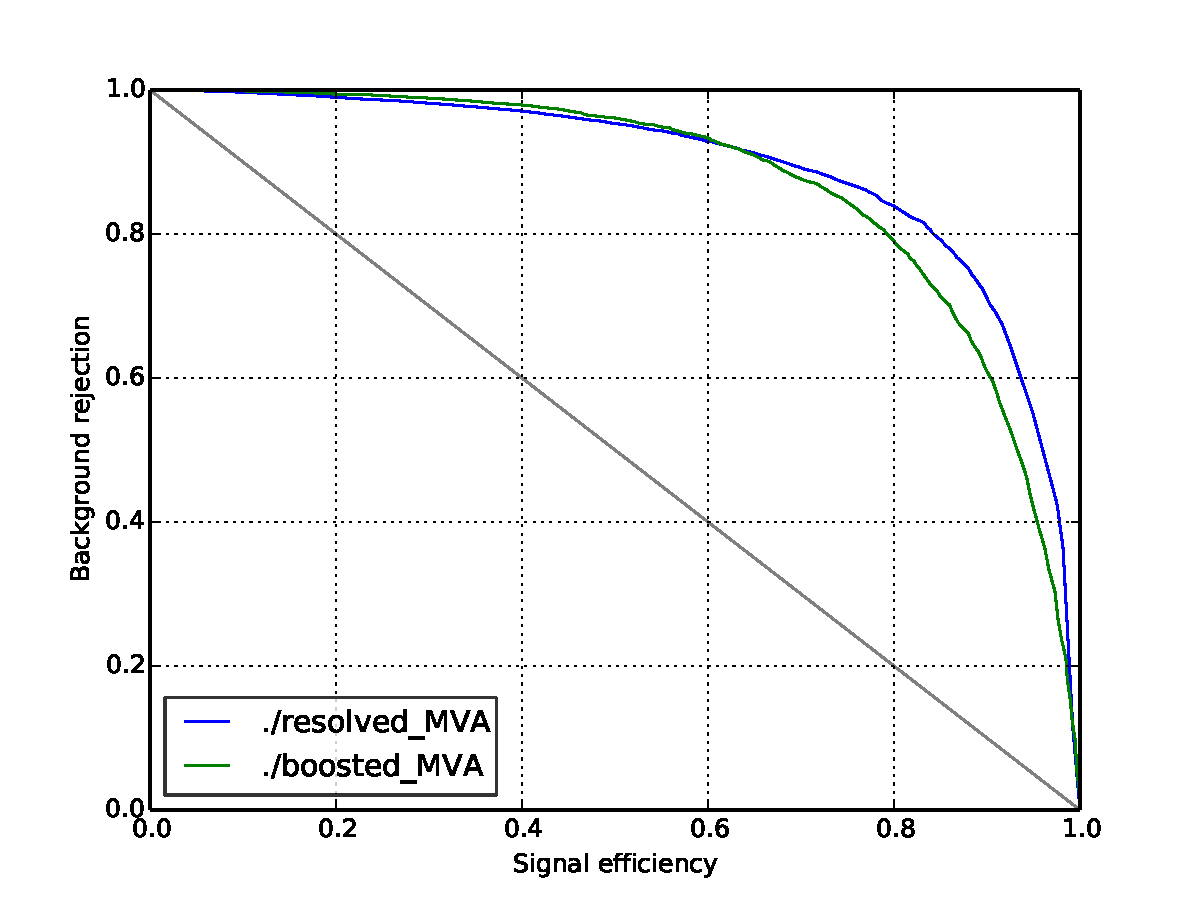
\includegraphics[width=0.95\textwidth]{plots/example_roc.pdf}
\caption{ROC curve for the neural network discriminant in the boosted (green) and resolved (blue) cases.}
\label{fig:exampleroc}
\end{center}
\end{figure}

\begin{figure}[h]
\begin{center}
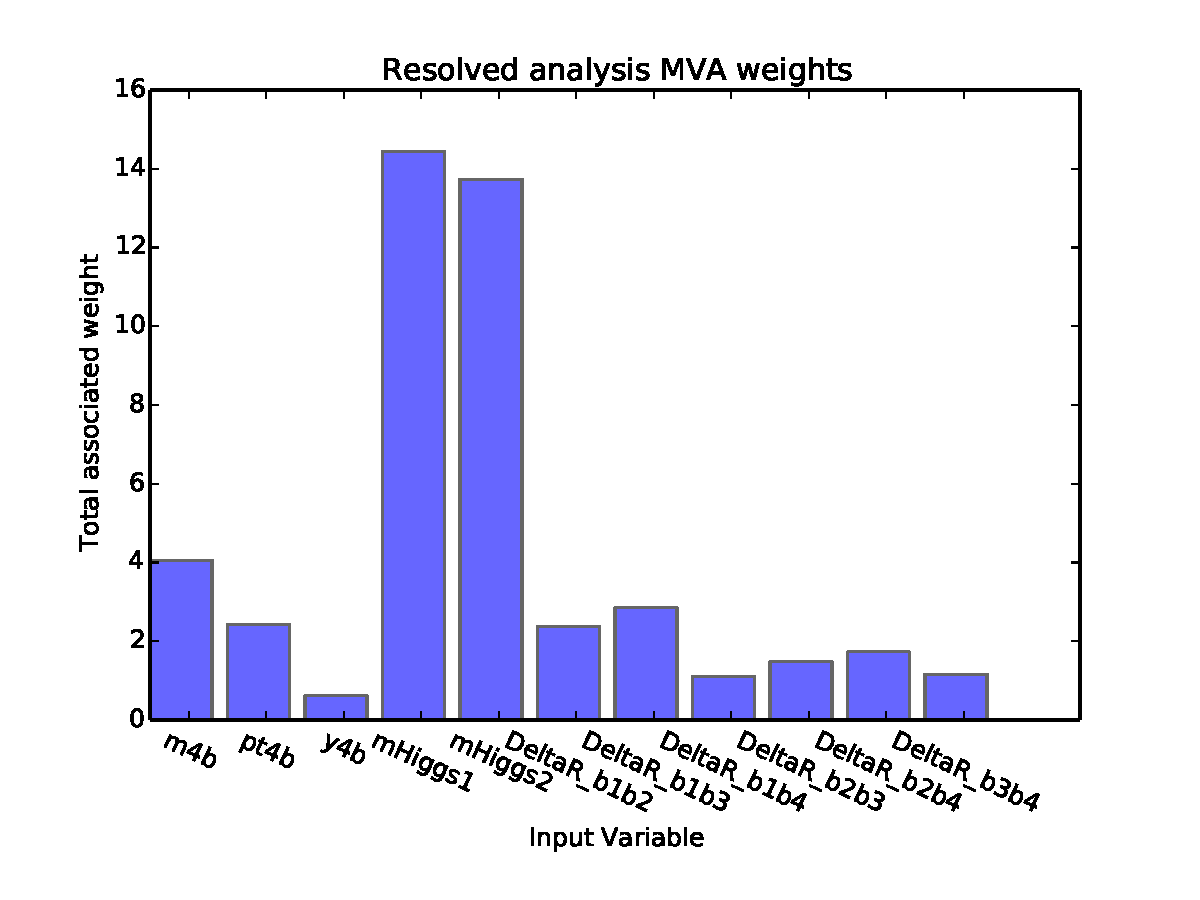
\includegraphics[width=1\textwidth]{plots/nnweights_res.pdf}
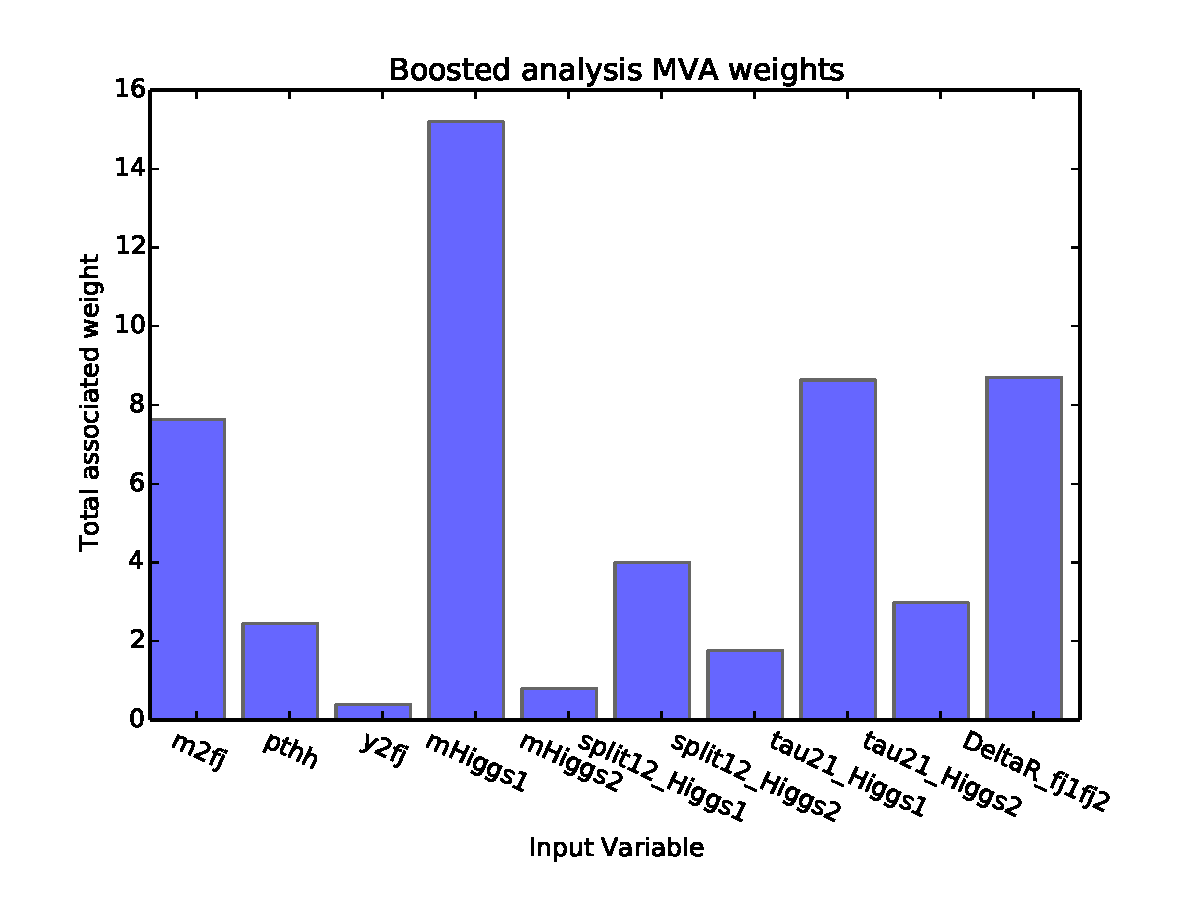
\includegraphics[width=1\textwidth]{plots/nnweights_boost.pdf}
\caption{Distribution of weights per input variable in the final ANN analysis. The above figure shows the weight distribution in the case of the resolved analysis, while the lower plot shows the boosted analysis.}
\label{fig:nnweights}
\end{center}
\end{figure}
\clearpage

Figure~\ref{fig:nnweights} demonstrates that the dijet invariant mass is a crucial variable for the resolved analysis MVA. As no detector effects were modelled in this analysis, it is reasonable to assume that the MVA has greater discriminating power than would be feasible in a real analysis. To investigate this, we now consider a variant of the analysis used in Table~\ref{tab:resCutflow} where the $m_H$ window criterion has been relaxed to $80 < m_H < 170$. Firstly the same analysis is repeated with the larger $m_H$ window. This is then compared to the same analysis but with a Gaussian smearing with $\sigma=10$ GeV applied to the dijet invariant mass used in the MVA. In the left panel of Figure~\ref{fig:invMsmear} the smearing is demonstrated. Despite the smearing, the MVA applied to this analysis still vastly prefers the dijet masses as discriminators, as is demonstrated in the right panel of Figure~\ref{fig:invMsmear}.
            
\begin{figure}[h!]
\begin{center}
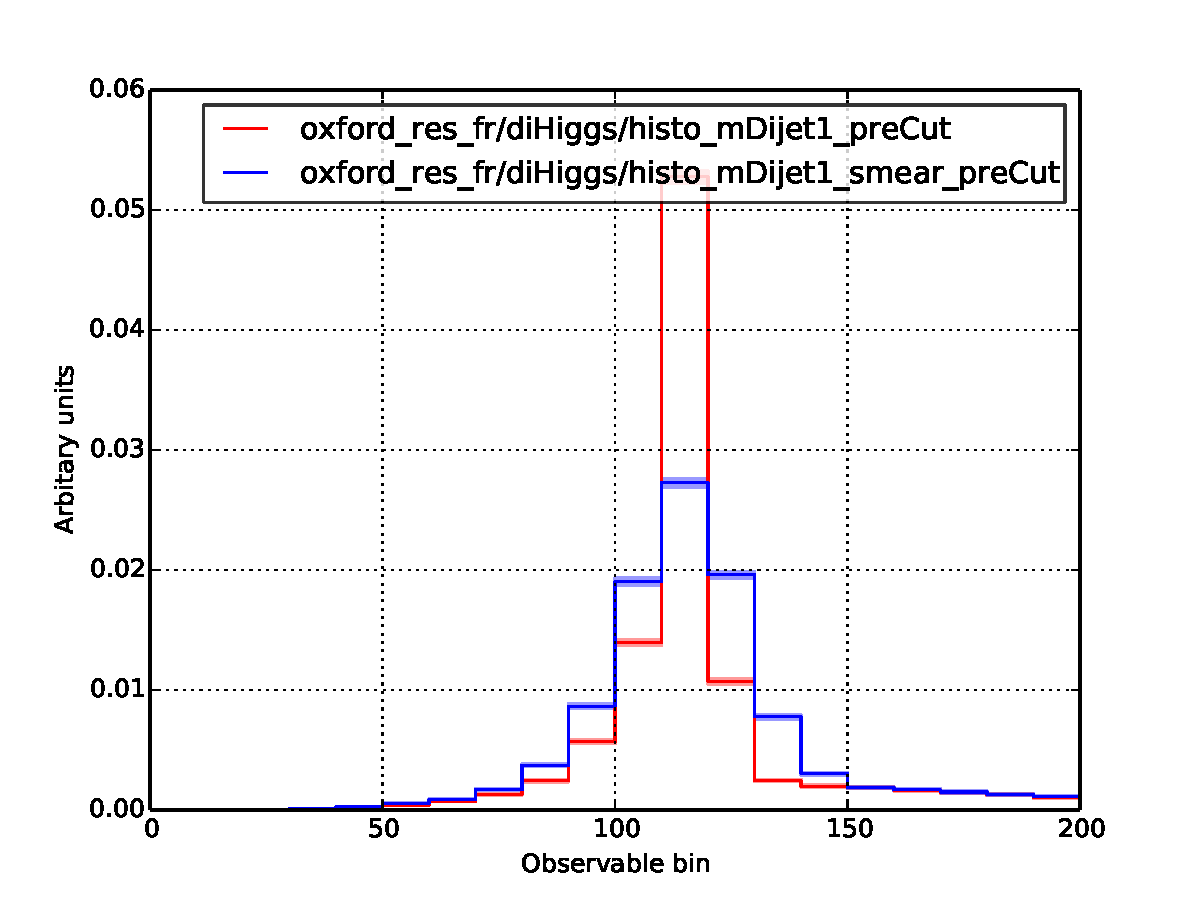
\includegraphics[width=0.49\textwidth]{plots/Msmear/histo_mass_smear_precut.pdf}
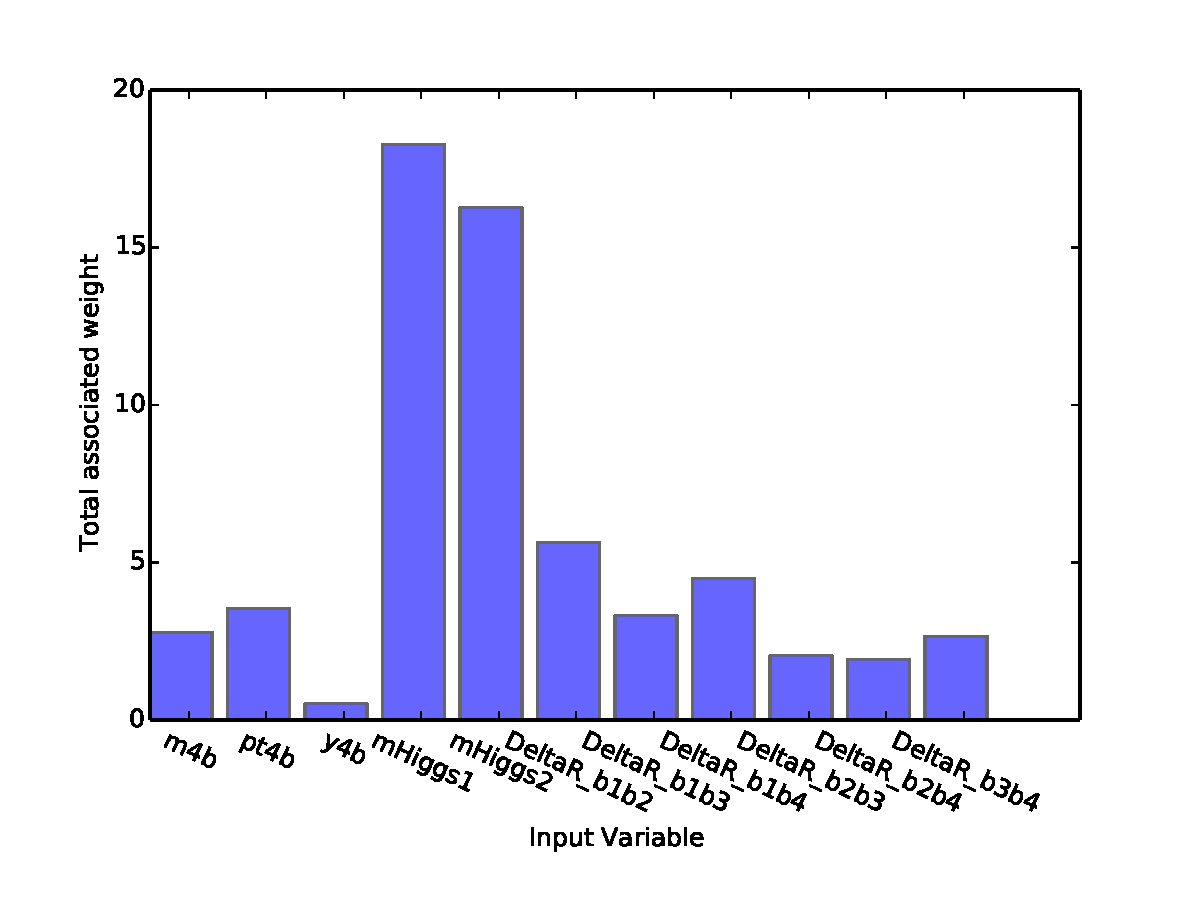
\includegraphics[width=0.49\textwidth]{plots/Msmear/nnweights.pdf}
\caption{The left figure demonstrates the gaussian smearing applied to the dijet invariant mass distribution. The right figure demonstrates the ANN weight distribution in the MVA.}
\label{fig:invMsmear}
\end{center}
\end{figure}

While the MVA still derives most of it's discriminating power from the dijet masses, the smearing reduces it's effectiveness considerably. In Figure \ref{fig:smearedROC} the ROC curves of the MVA applied to the smeared and unsmeared distributions are shown, where it is clear that the overall performance of the MVA is significantly hampered by the smeared invariant masses. This is echoed in the resulting significance of the analysis as demonstrated in Figure~\ref{fig:smearedSB}

\begin{figure}[h]
\begin{center}
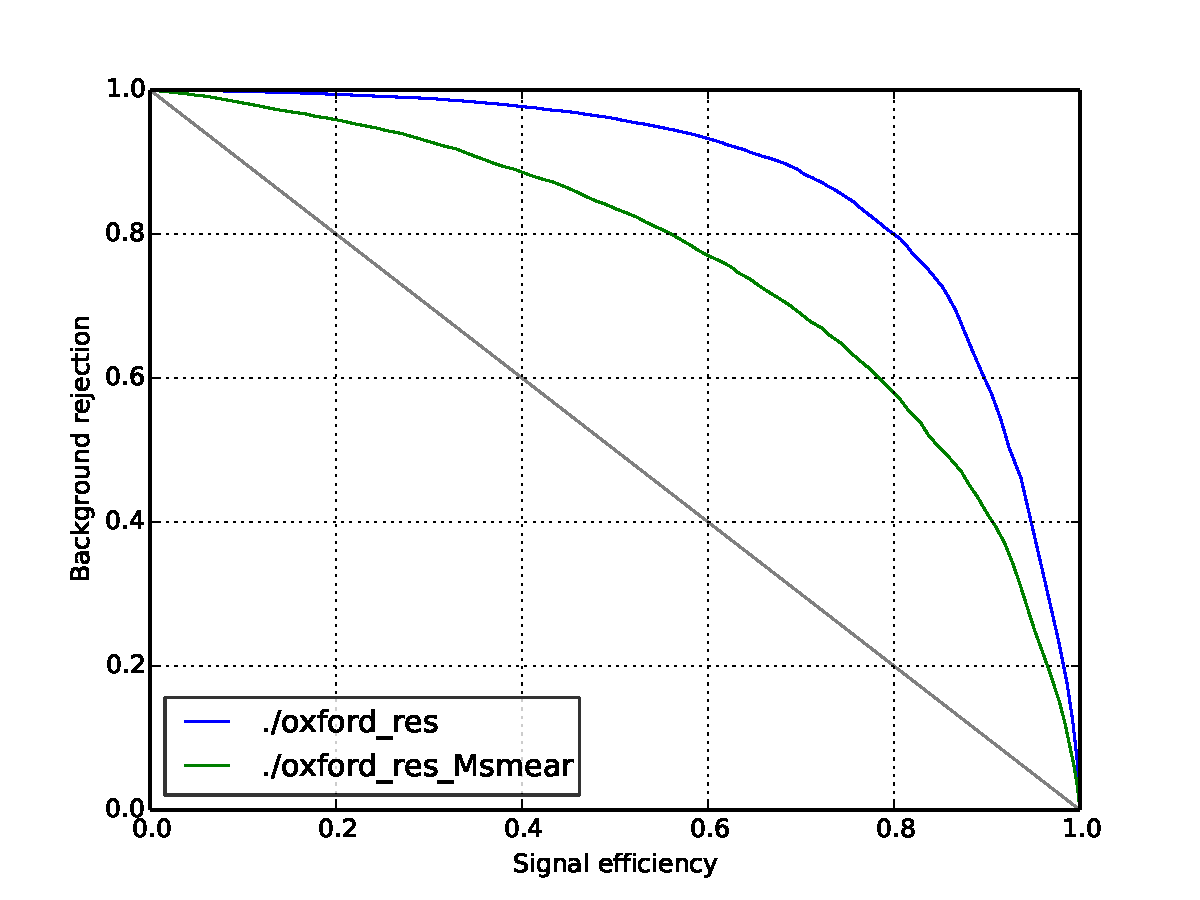
\includegraphics[width=0.89\textwidth]{plots/Msmear/roc.pdf}
\caption{ROC curves of the MVA applied with the unsmeared (blue) and smeared (green) dijet invariant mass distributions.}
\label{fig:smearedROC}
\end{center}
\end{figure}
            
       
\begin{figure}[h]
\begin{center}
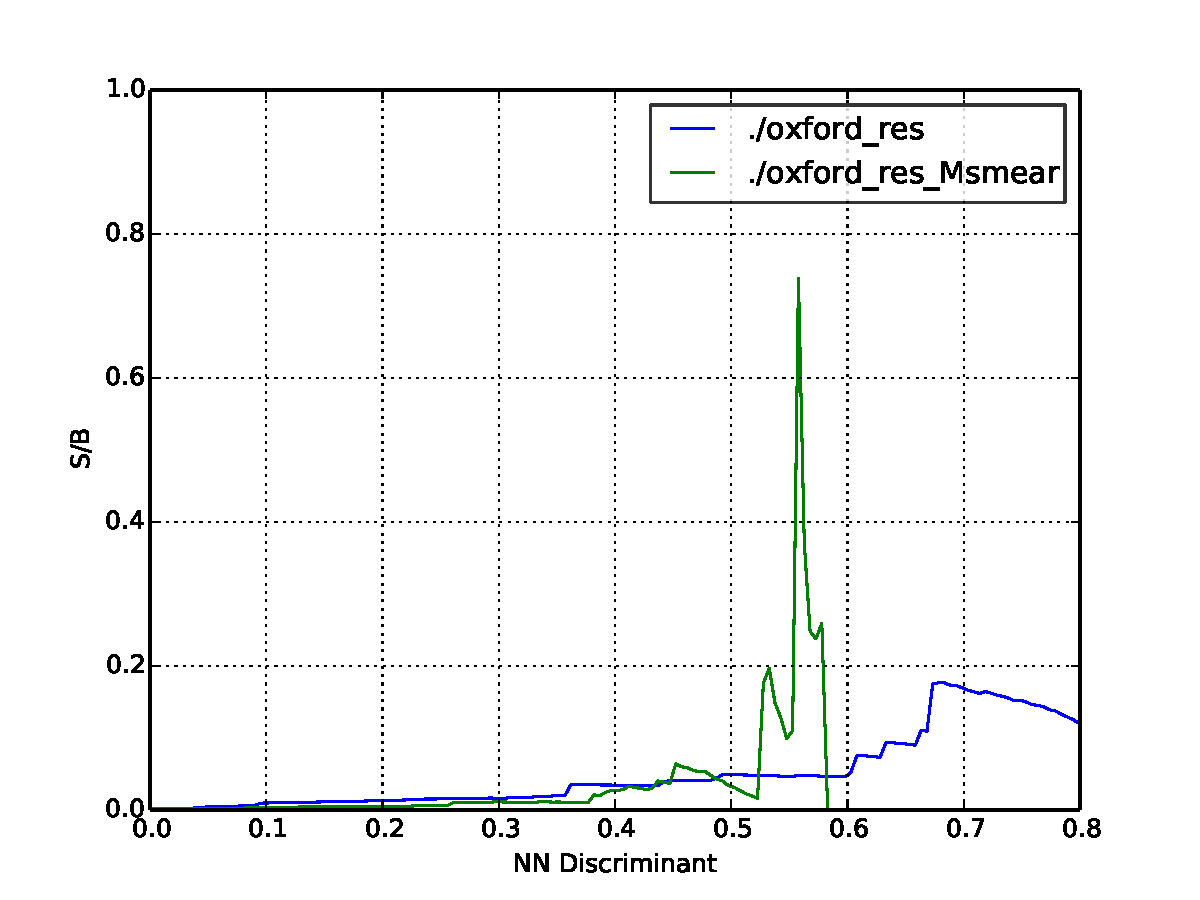
\includegraphics[width=0.49\textwidth]{plots/Msmear/sb.pdf}
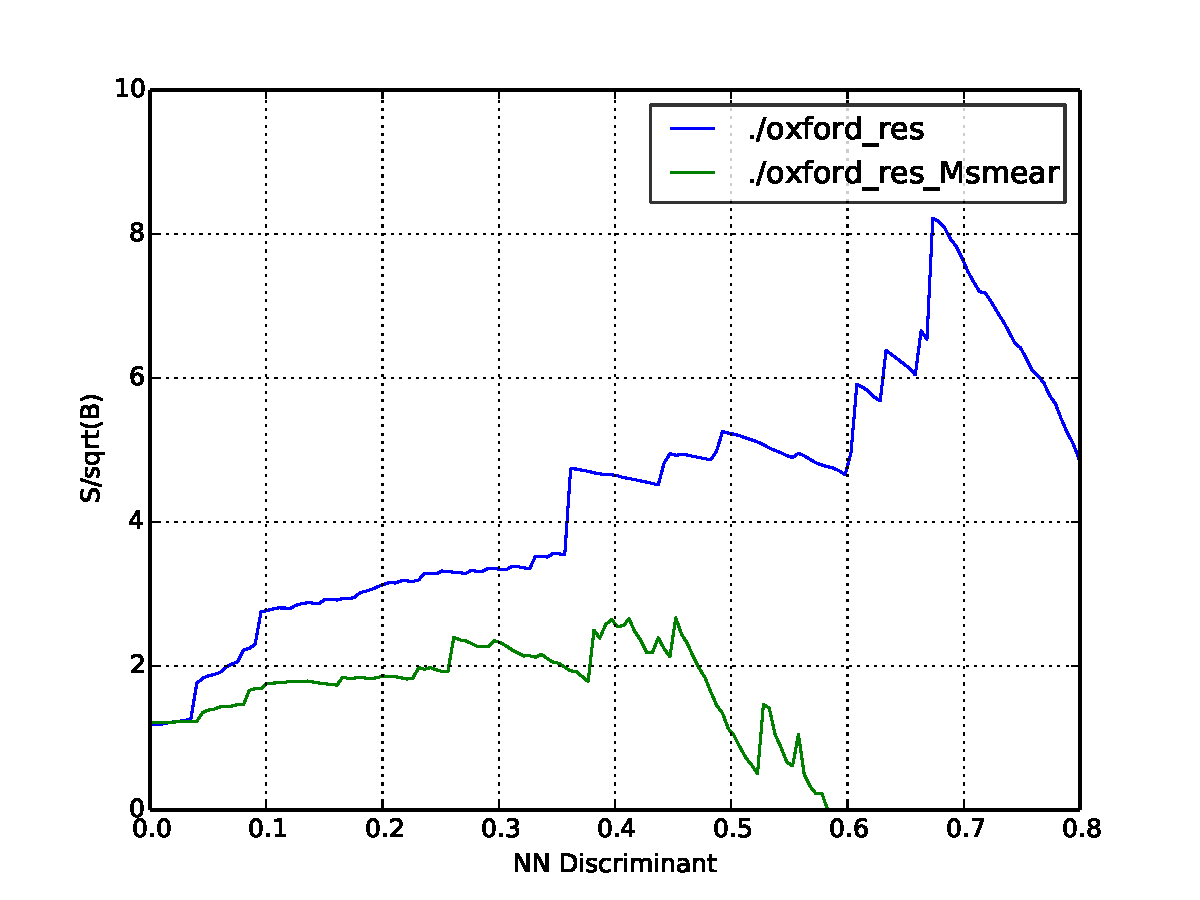
\includegraphics[width=0.49\textwidth]{plots/Msmear/ssb.pdf}
\caption{$S/B$ and $S\sqrt{B}$ (HL\-LHC) for the MVA applied to the unsmeared (blue) and smeared (green) dijet invariant mass distributions.}
\label{fig:smearedSB}
\end{center}
\end{figure}
\clearpage

\section{Conclusion}



% \Acknowledgements


\begin{thebibliography}{1}

%\cite{Alwall:2014hca}
\bibitem{Alwall:2014hca}
  J.~Alwall, R.~Frederix, S.~Frixione, V.~Hirschi, F.~Maltoni, O.~Mattelaer, H.-S.~Shao and T.~Stelzer {\it et al.},
  %``The automated computation of tree-level and next-to-leading order differential cross sections, and their matching to parton shower simulations,''
  JHEP {\bf 1407} (2014) 079
  [arXiv:1405.0301 [hep-ph]].
  %%CITATION = ARXIV:1405.0301;%%
  %168 citations counted in INSPIRE as of 19 Jan 2015

%\cite{Wardrope:2014kya}
\bibitem{Wardrope:2014kya}
  D.~Wardrope, E.~Jansen, N.~Konstantinidis, B.~Cooper, R.~Falla and N.~Norjoharuddeen,
  ``Non-resonant Higgs pair production in the $b\overline{b}b\overline{b}$ final state at the LHC,''
  arXiv:1410.2794 [hep-ph].
  %%CITATION = ARXIV:1410.2794;%%


  \end{thebibliography}


%%%%%%%%%%%%%%%%%%%%%%%%%%%%%%%%%%
%%%%%%%%%%%%%%%%%%%%%%%%%%%%%%%%%%
\clearpage
\appendix
\section{Event sample runcards}
\label{app:runcards}
\subsection {Background: QCD 4b}
\begin{verbatim}
(run){
  EVENTS 3M;
  EVENT_GENERATION_MODE U;
  ME_SIGNAL_GENERATOR Comix;

  EVENT_OUTPUT HepMC_Short[SHERPA_QCD_4b];

  BEAM_1 2212; BEAM_ENERGY_1 7000;
  BEAM_2 2212; BEAM_ENERGY_2 7000;

  FRAGMENTATION=Off # disable hadronisation
  MI_HANDLER=None # disable multiple parton interactions

  SCF:=1; ### default scale factor
  SCALES VAR{SCF*H_T2/4};

  PDF_LIBRARY LHAPDFSherpa;
  PDF_SET NNPDF30_lo_as_0118_nf_4.LHgrid;
  PDF_SET_VERSION 0;

  MASSIVE[5] 1;
  MASS[5] 4.75;

}(run);
(processes){
  Process 93 93 -> 5 -5 5 -5;
  Order_EW 0;
  End process;

}(processes);
(selector){
  PT 5 20 7000
  PT -5 20 7000
  PseudoRapidity 5 -3.0 3.0
  PseudoRapidity -5 -3.0 3.0

  DeltaR 5 5 0.1 10000
  DeltaR 5 -5 0.1 10000
  DeltaR -5 -5 0.1 10000

}(selector);
\end{verbatim}

\subsection {Background: QCD 2b2j}
\begin{verbatim}
(run){
  EVENTS 3M;
  EVENT_GENERATION_MODE U;
  ME_SIGNAL_GENERATOR Comix;

  EVENT_OUTPUT HepMC_Short[SHERPA_QCD_2b2j];

  BEAM_1 2212; BEAM_ENERGY_1 7000;
  BEAM_2 2212; BEAM_ENERGY_2 7000;

  FRAGMENTATION=Off # disable hadronisation
  MI_HANDLER=None # disable multiple parton interactions

  SCF:=1; ### default scale factor
  SCALES VAR{SCF*H_T2/4};

  PDF_LIBRARY LHAPDFSherpa;
  PDF_SET NNPDF30_lo_as_0118_nf_4.LHgrid;
  PDF_SET_VERSION 0;

  MASSIVE[5] 1;
  MASS[5] 4.75;

}(run);
(processes){
  Process 93 93 -> 93 93 5 -5;
  Order_EW 0;
  End process;

}(processes);
(selector){
  PT 5 20 7000
  PT -5 20 7000
  PseudoRapidity 5 -3 3
  PseudoRapidity -5 -3 3

  PT 93 20 7000
  PseudoRapidity 93 -3 3

  DeltaR 93 93 0.1 10000
  DeltaR 5 93 0.1 10000
  DeltaR -5 93 0.1 10000
  DeltaR 5 5 0.1 10000
  DeltaR -5 5 0.1 10000
  DeltaR -5 -5 0.1 10000
}(selector);
\end{verbatim}

\subsection {Background: QCD 4j}
\begin{verbatim}
(run){
  EVENTS 3M;
  EVENT_GENERATION_MODE U;
  ME_SIGNAL_GENERATOR Comix;

  EVENT_OUTPUT HepMC_Short[SHERPA_QCD_4j];

  BEAM_1 2212; BEAM_ENERGY_1 7000;
  BEAM_2 2212; BEAM_ENERGY_2 7000;

  FRAGMENTATION=Off # disable hadronisation
  MI_HANDLER=None # disable multiple parton interactions

  SCF:=1; ### default scale factor
  SCALES VAR{SCF*H_T2/4};

  PDF_LIBRARY LHAPDFSherpa;
  PDF_SET NNPDF30_lo_as_0118_nf_4.LHgrid;
  PDF_SET_VERSION 0;

  MASSIVE[5] 1;
  MASS[5] 4.75;

}(run);

(processes){
  Process 93 93 -> 93 93 93 93;
  Order_EW 0;
  End process;
}(processes);

(selector){
  PT 93 20 7000
  PseudoRapidity 93 -3 3
  DeltaR 93 93 0.1 10000
}(selector);
\end{verbatim}

\subsection {Background: QCD ttbar}
\begin{verbatim}
(run){
  EVENTS 3M;
  EVENT_GENERATION_MODE U;
  ME_SIGNAL_GENERATOR Comix;

  EVENT_OUTPUT HepMC_Short[SHERPA_QCD_ttbar];

  BEAM_1 2212; BEAM_ENERGY_1 7000;
  BEAM_2 2212; BEAM_ENERGY_2 7000;

  FRAGMENTATION=Off # disable hadronisation
  MI_HANDLER=None # disable multiple parton interactions

  SCF:=1; ### default scale factor
  SCALES VAR{SCF*H_T2/4};

  PDF_LIBRARY LHAPDFSherpa;
  PDF_SET NNPDF30_lo_as_0118_nf_4.LHgrid;
  PDF_SET_VERSION 0;

  MASSIVE[5] 1;
  MASS[5] 4.75;

  # Stable mode 0 specified that both particle and antiparticle are unstable
  STABLE[6] = 0;
  STABLE[24] = 0; 

  # Enable only fully hadronic decay modes
  HARD_DECAYS=1;   
  HDH_NO_DECAY={24,12,-11}|{24,14,-13}|{24,16,-15}|{-24,-12,11}|{-24,-14,13}|{-24,-16,15};

}(run);

(processes){
  Process 93 93 -> 6 -6;
  Order_EW 0;
  End process;
}(processes);

(selector){
  PT 6 20 7000
  PT -6 20 7000
  PseudoRapidity 6 -3 3
  PseudoRapidity -6 -3 3
  DeltaR 6 -6 0.1 10000
}(selector);
\end{verbatim}

\clearpage
\section{Decay tables for $t\bar{t}$}

\begin{verbatim}
Decay table for : W+.
Total width:                  2.10561 GeV
Flavour width:                2.06 GeV
----------------------------------------
{24,2,-1}         W+ --> u db              0.702203   GeV, BR= 33.3492 %
{24,4,-3}         W+ --> c sb              0.701546   GeV, BR= 33.318 %
{24,12,-11}       W+ --> nu_e e+           0.234068   GeV, BR= 11.1164 %
{24,14,-13}       W+ --> nu_mu mu+         0.234066   GeV, BR= 11.1163 %
{24,16,-15}       W+ --> nu_tau tau+       0.233725   GeV, BR= 11.1001 %
----------------------------------------

Decay table for : W-.
Total width:                  2.10561 GeV
Flavour width:                2.06 GeV
----------------------------------------
{-24,-2,1}        W- --> ub d              0.702203   GeV, BR= 33.3492 %
{-24,-4,3}        W- --> cb s              0.701546   GeV, BR= 33.318 %
{-24,-12,11}      W- --> nu_eb e-          0.234068   GeV, BR= 11.1164 %
{-24,-14,13}      W- --> nu_mub mu-        0.234066   GeV, BR= 11.1163 %
{-24,-16,15}      W- --> nu_taub tau-      0.233725   GeV, BR= 11.1001 %
----------------------------------------

Decay table for : t.
Total width:                  1.59689 GeV
Flavour width:                1.5 GeV
----------------------------------------
{6,24,5}          t --> W+ b               1.59689    GeV, BR= 100   %
----------------------------------------

Decay table for : tb.
Total width:                  1.59689 GeV
Flavour width:                1.5 GeV
----------------------------------------
{-6,-24,-5}       tb --> W- bb             1.59689    GeV, BR= 100   %

\end{verbatim}

%%%%%%%%%%%%%%%%%%%%%%%%%%%%%%%%%%
%%%%%%%%%%%%%%%%%%%%%%%%%%%%%%%%%%

\end{document}

